\documentclass[]{book}
\usepackage{lmodern}
\usepackage{amssymb,amsmath}
\usepackage{ifxetex,ifluatex}
\usepackage{fixltx2e} % provides \textsubscript
\ifnum 0\ifxetex 1\fi\ifluatex 1\fi=0 % if pdftex
  \usepackage[T1]{fontenc}
  \usepackage[utf8]{inputenc}
\else % if luatex or xelatex
  \ifxetex
    \usepackage{mathspec}
  \else
    \usepackage{fontspec}
  \fi
  \defaultfontfeatures{Ligatures=TeX,Scale=MatchLowercase}
\fi
% use upquote if available, for straight quotes in verbatim environments
\IfFileExists{upquote.sty}{\usepackage{upquote}}{}
% use microtype if available
\IfFileExists{microtype.sty}{%
\usepackage{microtype}
\UseMicrotypeSet[protrusion]{basicmath} % disable protrusion for tt fonts
}{}
\usepackage[margin=1in]{geometry}
\usepackage{hyperref}
\hypersetup{unicode=true,
            pdftitle={analizaR datos políticos},
            pdfauthor={Francisco Urdinez y Andrés Cruz},
            pdfborder={0 0 0},
            breaklinks=true}
\urlstyle{same}  % don't use monospace font for urls
\usepackage{natbib}
\bibliographystyle{apalike}
\usepackage{color}
\usepackage{fancyvrb}
\newcommand{\VerbBar}{|}
\newcommand{\VERB}{\Verb[commandchars=\\\{\}]}
\DefineVerbatimEnvironment{Highlighting}{Verbatim}{commandchars=\\\{\}}
% Add ',fontsize=\small' for more characters per line
\usepackage{framed}
\definecolor{shadecolor}{RGB}{248,248,248}
\newenvironment{Shaded}{\begin{snugshade}}{\end{snugshade}}
\newcommand{\KeywordTok}[1]{\textcolor[rgb]{0.13,0.29,0.53}{\textbf{#1}}}
\newcommand{\DataTypeTok}[1]{\textcolor[rgb]{0.13,0.29,0.53}{#1}}
\newcommand{\DecValTok}[1]{\textcolor[rgb]{0.00,0.00,0.81}{#1}}
\newcommand{\BaseNTok}[1]{\textcolor[rgb]{0.00,0.00,0.81}{#1}}
\newcommand{\FloatTok}[1]{\textcolor[rgb]{0.00,0.00,0.81}{#1}}
\newcommand{\ConstantTok}[1]{\textcolor[rgb]{0.00,0.00,0.00}{#1}}
\newcommand{\CharTok}[1]{\textcolor[rgb]{0.31,0.60,0.02}{#1}}
\newcommand{\SpecialCharTok}[1]{\textcolor[rgb]{0.00,0.00,0.00}{#1}}
\newcommand{\StringTok}[1]{\textcolor[rgb]{0.31,0.60,0.02}{#1}}
\newcommand{\VerbatimStringTok}[1]{\textcolor[rgb]{0.31,0.60,0.02}{#1}}
\newcommand{\SpecialStringTok}[1]{\textcolor[rgb]{0.31,0.60,0.02}{#1}}
\newcommand{\ImportTok}[1]{#1}
\newcommand{\CommentTok}[1]{\textcolor[rgb]{0.56,0.35,0.01}{\textit{#1}}}
\newcommand{\DocumentationTok}[1]{\textcolor[rgb]{0.56,0.35,0.01}{\textbf{\textit{#1}}}}
\newcommand{\AnnotationTok}[1]{\textcolor[rgb]{0.56,0.35,0.01}{\textbf{\textit{#1}}}}
\newcommand{\CommentVarTok}[1]{\textcolor[rgb]{0.56,0.35,0.01}{\textbf{\textit{#1}}}}
\newcommand{\OtherTok}[1]{\textcolor[rgb]{0.56,0.35,0.01}{#1}}
\newcommand{\FunctionTok}[1]{\textcolor[rgb]{0.00,0.00,0.00}{#1}}
\newcommand{\VariableTok}[1]{\textcolor[rgb]{0.00,0.00,0.00}{#1}}
\newcommand{\ControlFlowTok}[1]{\textcolor[rgb]{0.13,0.29,0.53}{\textbf{#1}}}
\newcommand{\OperatorTok}[1]{\textcolor[rgb]{0.81,0.36,0.00}{\textbf{#1}}}
\newcommand{\BuiltInTok}[1]{#1}
\newcommand{\ExtensionTok}[1]{#1}
\newcommand{\PreprocessorTok}[1]{\textcolor[rgb]{0.56,0.35,0.01}{\textit{#1}}}
\newcommand{\AttributeTok}[1]{\textcolor[rgb]{0.77,0.63,0.00}{#1}}
\newcommand{\RegionMarkerTok}[1]{#1}
\newcommand{\InformationTok}[1]{\textcolor[rgb]{0.56,0.35,0.01}{\textbf{\textit{#1}}}}
\newcommand{\WarningTok}[1]{\textcolor[rgb]{0.56,0.35,0.01}{\textbf{\textit{#1}}}}
\newcommand{\AlertTok}[1]{\textcolor[rgb]{0.94,0.16,0.16}{#1}}
\newcommand{\ErrorTok}[1]{\textcolor[rgb]{0.64,0.00,0.00}{\textbf{#1}}}
\newcommand{\NormalTok}[1]{#1}
\usepackage{longtable,booktabs}
\usepackage{graphicx,grffile}
\makeatletter
\def\maxwidth{\ifdim\Gin@nat@width>\linewidth\linewidth\else\Gin@nat@width\fi}
\def\maxheight{\ifdim\Gin@nat@height>\textheight\textheight\else\Gin@nat@height\fi}
\makeatother
% Scale images if necessary, so that they will not overflow the page
% margins by default, and it is still possible to overwrite the defaults
% using explicit options in \includegraphics[width, height, ...]{}
\setkeys{Gin}{width=\maxwidth,height=\maxheight,keepaspectratio}
\IfFileExists{parskip.sty}{%
\usepackage{parskip}
}{% else
\setlength{\parindent}{0pt}
\setlength{\parskip}{6pt plus 2pt minus 1pt}
}
\setlength{\emergencystretch}{3em}  % prevent overfull lines
\providecommand{\tightlist}{%
  \setlength{\itemsep}{0pt}\setlength{\parskip}{0pt}}
\setcounter{secnumdepth}{5}
% Redefines (sub)paragraphs to behave more like sections
\ifx\paragraph\undefined\else
\let\oldparagraph\paragraph
\renewcommand{\paragraph}[1]{\oldparagraph{#1}\mbox{}}
\fi
\ifx\subparagraph\undefined\else
\let\oldsubparagraph\subparagraph
\renewcommand{\subparagraph}[1]{\oldsubparagraph{#1}\mbox{}}
\fi

%%% Use protect on footnotes to avoid problems with footnotes in titles
\let\rmarkdownfootnote\footnote%
\def\footnote{\protect\rmarkdownfootnote}

%%% Change title format to be more compact
\usepackage{titling}

% Create subtitle command for use in maketitle
\newcommand{\subtitle}[1]{
  \posttitle{
    \begin{center}\large#1\end{center}
    }
}

\setlength{\droptitle}{-2em}
  \title{analizaR datos políticos}
  \pretitle{\vspace{\droptitle}\centering\huge}
  \posttitle{\par}
  \author{Francisco Urdinez y Andrés Cruz}
  \preauthor{\centering\large\emph}
  \postauthor{\par}
  \predate{\centering\large\emph}
  \postdate{\par}
  \date{2017-12-20}

\usepackage{booktabs}
\usepackage{amsthm}
\makeatletter
\def\thm@space@setup{%
  \thm@preskip=8pt plus 2pt minus 4pt
  \thm@postskip=\thm@preskip
}
\makeatother

\begin{document}
\maketitle

{
\setcounter{tocdepth}{1}
\tableofcontents
}
\chapter{Prefacio}\label{prefacio}


\includegraphics[width=0.6\linewidth]{images/tapa}

Este libro nació haciendo análisis de datos políticos. Es decir, es hijo
de la praxis. Por ello su naturaleza es aplicada, y tiene su foco puesto
en ser una caja de herramientas para el lector. AnalizaR datos políticos
está pensado para ser un manual de referencia que podrá ser consultado
tanto por un estudiante universitario viviendo en Bogotá, como por un
consultor político viviendo en México DF o un o funcionário público en
Brasilia, todos con la necesidad de transformar sus bases de datos en
conclusiones sustantivas y fácilmente interpretables.

Trabajando juntos en la cátedra de Análisis Cuantitativo de Datos II del
Instituto de Ciencia Política de la Universidad Católica de Chile
encontramos que ni aquí, ni en otras universidades de la región, había
material didáctico y aplicado hecho en casa para enseñar a nuestros
alumnos de ciencia política cómo extraer conclusiones a partir de datos
duros. Todo el material utilizado en nuestra cátedra era publicado en
inglés, por politólogos anglosajones trabajando en universidades
anglosajonas. Por ello analizaR datos políticos tiene como público
imaginario al politólogo latinoamericano, ya sea alumno de pregrado o
posgrado, o ya en el mercado. Hemos querido que nuestro libro esté
disponible en español y portugués, y esto lo hace extensible a otras
universidades de realidades similares fuera de América Latina, como en
los países lusófonos de África y en la región ibérica.

Las universidades latinoamericanas han hecho grandes esfuerzos en que
sus alumnos de politología se alfabeticen en herramientas estadísticas y
de análisis de datos, algo que hasta hace diez años era algo poco
frecuente. Hoy las cinco mejores universidades de la región, según el
ranking de Times Higher Eductaion, tienen cursos de análisis
cuantitativo de datos en sus programas de ciencia política. Algunos
departamentos, como el Departamento de Ciencia Política de la
Universidad de São Paulo, que co-organiza la escuela de verano de IPSA
en métodos, o el Instituto de Ciencia Política de la Universidad
Católica de Chile, que organiza su escuela de verano en métodos mixtos,
han hecho esfuerzos por exponer a sus alumnos a profesores
norteamericanos y europeos, quienes cuentan con muchas décadas de
tradición cuantitativa en sus programas. Entendemos que, hoy por hoy,
ningún politólogo puede salir al mercado laboral sin saber utilizar con
holgura software de análisis cuantitativo, y es a esa demanda a la que
apuntamos aquí.

Ahora mismo, R es probablemente la mejor opción que el mercado provee
para análisis estadístico de datos. Esto puede ser sorpresivo para un
lector recién salido de una máquina del tiempo: hace diez años, o tal
vez menos, R era simplemente mirado como la alternativa gratis a los
programas comerciales de verdad, que sí podían realizar análisis
cuantitativo serio. Sin embargo, esto ha cambiado drásticamente en los
últimos años. La figura 1 muestra las tendencias de búsqueda en Google
en América Latina para los programas más comúnmente utilizados en
ciencia. R ha pasado a ocupar un lugar en el mercado que hace 15 años le
correspondía a SPSS, y los programas de nicho -como Stata y Minitab- son
cada vez menos buscados. La tendencia sugiere que R será cada vez más
popular en la ciencia latinoamericana, siguiendo una tendencia global.

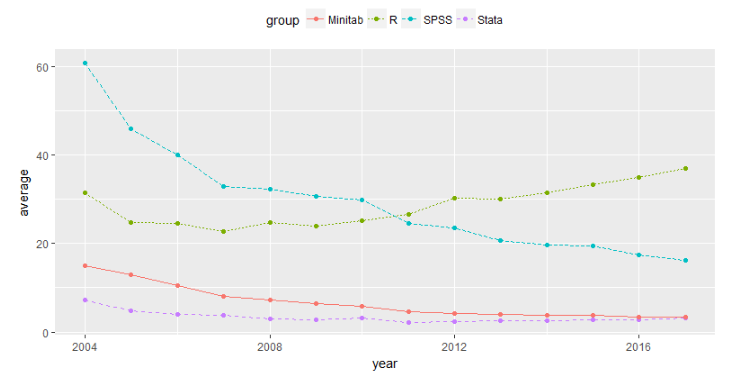
\includegraphics[width=1.2\linewidth]{images/fig_1_1} Nota: Elaborado
por los autores usando el paquete ggplot2 de R, y datos extraídos de
Google Trends. Los datos corresponden a promedios anuales para países
latinoamericanos en el sector ``ciencia''.

El modelo de software libre en el que se basa R ---con licencias de
derechos de autor permisivas, que ponen prácticamente todas las
herramientas en forma gratuita a disposición del público, tanto para su
uso como para su reformulación--- finalmente rindió frutos. Una activa
comunidad de desarrolladores se ha anclado en R, añadiéndole nuevas
funcionalidades que lo han dotado de elegancia, simplicidad y
flexibilidad. R ya no solo brilla en la generación de modelos
estadísticos, sino que hoy es hogar de un vasto universo de herramientas
que permite al usuario importar, ordenar, transformar, visualizar,
modelar y comunicar los datos que le interesen, sin tener que cambiar de
herramienta. Es esta la novedad tecnológica que queremos acercar al
lector interesado en el análisis político, con la esperanza de que
contribuya a optimizar el proceso entre la pregunta que le quita el
sueño (y/o le promete el pan) y su solución. Esto sin desconocer, claro
está, que el beneficio inicial de R, el que estaba incluso cuando nadie
quisiera usarlo si no era a regañadientes, permanece. Sabemos que el
lector ---y tal vez su casa de estudios--- agradecerá la amable
coincidencia de que el mejor software disponible en términos de calidad
es también el mejor para su bolsillo.

\section{Agradecimientos}\label{agradecimientos}

Por ahora nadie.

\chapter{Introducción}\label{introduccion}

El análisis cuantitativo de datos es una de las tantas herramientas que
los investigadores tenemos para abordar las preguntas que nos interesan,
ya sea en el mundo profesional o la academia (o ``por amor al arte'' en
muy encendidas noches de viernes, por qué no). Es por esto que analizaR
datos políticos tiene un fuerte énfasis en ejemplos politológicos
aplicados. Utilizar ejemplos de texto trillados e idealizados sobre
autitos o islas imaginarias sería una falta de respeto para el lector, a
quien sabemos ávido por ocupar las herramientas de este libro en las
preguntas de investigación política que le parecen importantes. Por el
contrario, queremos mostrar el potencial de dichas herramientas metiendo
las manos en la masa, con datos de verdad, investigaciones que colegas
ya han realizado y dificultades particulares de llevar el análisis de
datos a preguntas políticas.

\section{Organización del libro}\label{organizacion-del-libro}

El libro está organizado en tres secciones temáticas. Dentro de las
secciones, cada capítulo se esfuerza por resolver problemas puntuales,
balanceando teoría y práctica en R.

 La sección I está dedicada al manejo de datos. Lo ideal es que el
lector consiga algo más que mirar una base de datos con cara de no
entender nada. Introduciremos R desde su instalación y aprenderemos a
sacarle el jugo para obtener datos, conocerlos en profundidad,
transformarlos de acuerdo a las preguntas que nos interesan y
representarlos gráficamente en formas tanto funcionales como atractivas.

 Luego, en la sección II está el corazón del libro. Veremos cómo
responder a preguntas políticas desde una perspectiva estadística
---siempre podemos contestar desde la perspectiva de lo que nos dijo
nuestra abuelita, aunque esto suela ser menos serio---. En general, la
sección trata modelos estadísticos, que intentan explicar y predecir la
variación de ciertas variables (dependientes) de acuerdo a cómo varían
otras variables (independientes). Exploraremos distintos tipos de
modelos de acuerdo a las distintas formas de variables dependientes que
se encuentran comúnmente en la arena de lo político. Revisaremos cómo
interpretar resultados y presentarlos en forma clara y atractiva, cómo
elegir entre modelos competidores y cómo comprobar simplemente algunos
de los supuestos estadísticos necesarios para que los modelos funcionen.
Debemos notar que este no es un libro de econometría, claro está, por lo
que para cada modelo haremos referencia a trabajos más avanzados en
términos teóricos, con el fin de que el lector pueda profundizar por su
cuenta si cree que debe utilizar algún modelo en específico para
responder a sus preguntas de interés.

 Por último, en la sección III dejaremos el mundo ideal y nos
adentraremos en la resolución de problemas. Ya sea porque un colega nos
prestó su base y parece más bien una obra de arte surrealista o
simplemente porque la dificultad de los problemas a los que nos
enfrentamos deja corto a lo que aprendimos al principio del libro, aquí
presentaremos un popurrí de herramientas para que el lector integre en
su flujo de trabajo. Estas han sido seleccionadas desde nuestra
experiencia y son cuáles creemos las más requeridas en la práctica del
análisis de datos políticos.

\section{Prerrequisitos}\label{prerrequisitos}

Este libro está pensado para alumnos que más que brillantes son
motivados: el análisis cuantitativo de datos exige sobre todo tenacidad
y curiosidad. Es altamente deseable que el lector tenga nociones básicas
de matemática, probabilidad y/o estadística universitaria antes de leer
este libro, aun cuando nos esforzamos por mantenerlo lo más simple que
pudimos en dichas materias. En términos de hardware, prácticamente
cualquier computador moderno con acceso a internet será suficiente, pues
las herramientas que utilizaremos son más bien livianas. Todo el
software que utilizaremos es gratuito.

\chapter{R básico}\label{r-basico}

\section{Instalación}\label{instalacion}

\subsection{R}\label{r}

R (R Core Team, 2017) es un lenguaje de programación especialmente
desarrollado para realizar análisis estadístico. Una de sus principales
características, como se ha dejado a entrever en el prefacio, es que es
de \emph{código libre}: aparte de ser gratis, esto significa que las
licencias que protegen legalmente a R son muy permisivas. Al amparo de
esas licencias, miles de desarrolladores alrededor del mundo han añadido
su granito de arena a la usabilidad y atractivo de R. ¡En \emph{analizaR
datos políticos} le sacaremos el jugo a esa diversidad, intentando no
ser dispersos!

Instalar R es fácil, independiente de si el usuario utiliza Windows, Mac
o Linux. Basta con ingresar a \url{https://cran.r-project.org/} y seguir
las instrucciones de descarga a instalación (\emph{¿poner más en un
anexo?})

\subsection{RStudio}\label{rstudio}

Como dijimos, R es un lenguaje de programación. En términos informales,
es una forma ordenada de pedirle al computador que realice ciertas
operaciones. Esto significa que es posible usar R exclusivamente desde
una consola o terminal -las pantallas negras de los hackers de las
películas. Aunque esto tiene algunos atractivos -entre ellos, parecer
hacker-, en general queremos interfaces más amigables. Ahí es cuando
entra al ruedo RStudio, el programa de facto para utilizar R. Una vez
esté instalado, todos nuestros análisis ocurrirán dentro de RStudio,
que, para más remate, es también de código libre. Para instalar RStudio,
es necesario ya haber instalado R. Como para este, la descarga e
instalación es accesible en Windows, Mac y Linux. El link es
\url{https://www.rstudio.com/products/rstudio/download/\#download}
(\emph{¿poner más en un anexo?})

\section{Partes de RStudio}\label{partes-de-rstudio}

Si el lector consiguió descargar e instalar R y RStudio, bastará con
ingresar a RStudio para comenzar a trabajar. Se pillará con una pantalla
como esta (\emph{pulir! mejor fuente, fondo blanco}):

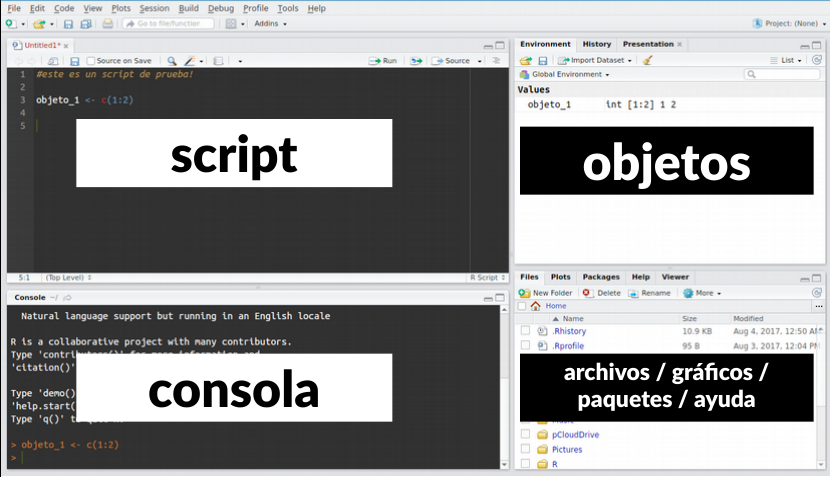
\includegraphics[width=1.2\linewidth]{00-images/fig_3_1}

La pantalla de RStudio se divide en cuatro paneles A continuación, vamos
a explicar sus funciones. La idea será familiarizar al lector con lo
básico de R en el camino.

\subsection{Consola}\label{consola}

El panel inferior izquierdo de RStudio. Es nuestro espacio de
comunicación directa con el computador, en el que le solicitamos,
hablando R, realizar tareas específicas. Llamaremos \textbf{comandos} a
estas solicitudes. Probemos correr un comando que realiza una operación
aritmética básica:

\begin{Shaded}
\begin{Highlighting}[]
\DecValTok{2} \OperatorTok{+}\StringTok{ }\DecValTok{2}
\end{Highlighting}
\end{Shaded}

\begin{verbatim}
## [1] 4
\end{verbatim}

Un truco importante de la consola es que con los botones de arriba y
abajo es posible navegar en el historial de comandos recientes.
Recomendamos al lector probar a realizar otros comandos con operaciones
aritméticas y volver atrás con los botones de arriba y abajo.

\emph{cambiar imagen de resumen}

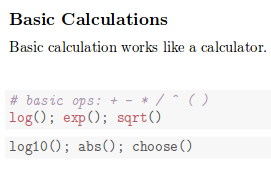
\includegraphics[width=0.8\linewidth]{00-images/fig_3_2}

Por ejemplo:

\begin{Shaded}
\begin{Highlighting}[]
\KeywordTok{sqrt}\NormalTok{(}\DecValTok{100}\NormalTok{) }\OperatorTok{-}\StringTok{ }\DecValTok{2}\OperatorTok{^}\DecValTok{3} \OperatorTok{*}\StringTok{ }\DecValTok{3}
\end{Highlighting}
\end{Shaded}

\begin{verbatim}
## [1] -14
\end{verbatim}

\subsection{Script}\label{script}

El panel superior izquierdo de RStudio. Puede describirse como una
suerte de ``bitácora de comandos''. Aunque la consola puede ser útil
para unos pocos comandos, análisis complejos requerirán que llevemos un
registro de nuestros comandos.

Para abrir un script nuevo, basta con presionar
\texttt{Ctrl\ +\ Shift\ +\ N} o ir a File \textgreater{} New File
\textgreater{} R Script (utilizar atajos de teclado suele ser una buena
idea, y no solo por el factor hacker \emph{footnote al anexo tips?}). La
pantalla en blanco de un nuevo script es similar a un bloc de notas en
blanco, con la particularidad de que cada línea debe pensarse como un
comando. El lector debe notar que escribir un comando en el script y
presionar \texttt{Enter} no consigue nada más que un salto de párrafo.
Para correr el comando de una línea basta con presionar
\texttt{Ctrl\ +\ Enter} (en el caso de Mac, \texttt{Cmd\ +\ Enter})
mientras se tiene el teclado en ella. ¡Es posible seleccionar múltiples
líneas/comandos a la vez y correrlas de una pasada con
\texttt{Ctrl\ +\ Enter}!

Es fundamental el dejar comentarios explicativos en nuestros scripts.
Esto no es solo relevante en el trabajo en grupo (el código ajeno puede
ser inentendible sin una guía clara), sino que también denota atención
por nuestros yo del futuro. En varias ocasiones nos ha tocado revisar
código que escribimos hace un par de meses, no entender nada, y maldecir
a nuestros yo del pasado por su poca consideración. A la hora de
interpretar comandos, R reconoce que todo lo que siga a un gato (o
\emph{hashtag}, en estos días) es un comentario. Así, hay dos formas de
dejar comentarios, como ``comandos estériles'' o como apéndices de
comandos funcionales:

\begin{Shaded}
\begin{Highlighting}[]
\CommentTok{# Este es un comando estéril. R sabe que es solo un comentario, por lo que no retorna nada.}
\end{Highlighting}
\end{Shaded}

\begin{Shaded}
\begin{Highlighting}[]
\DecValTok{2} \OperatorTok{+}\StringTok{ }\DecValTok{2} \CommentTok{# Este es un comando-apéndice. ¡R corre el comando hasta el gato y luego sabe que es un comentario!}
\end{Highlighting}
\end{Shaded}

\begin{verbatim}
## [1] 4
\end{verbatim}

Para guardar un script, basta con presionar \texttt{Ctrl\ +\ S} o
clickear File \textgreater{} Save.

\subsection{Objetos}\label{objetos}

El panel superior derecho de RStudio. Aunque tiene tres pestañas, la
gran estrella es ``Environment'', que sirve como registro para los
objetos que vayamos creando a medida que trabajamos. Una de las
características centrales de R es que permite almacenar objetos, para
luego correr comandos en ellos. La forma tipo para crear un objeto es
\texttt{nombre\_del\_objeto\ \textless{}-\ contenido}. Por ejemplo:

\begin{Shaded}
\begin{Highlighting}[]
\NormalTok{objeto_}\DecValTok{1}\NormalTok{ <-}\StringTok{ }\DecValTok{2} \OperatorTok{+}\StringTok{ }\DecValTok{2}
\end{Highlighting}
\end{Shaded}

El lector notará que en la pestaña ``Environment'' aparece un nuevo
objeto, objeto\_1. Este contiene \emph{el resultado} de 2 + 2. Es
posible preguntarle a R qué contiene un objeto simplemente corriendo su
nombre como si fuera un comando:

\begin{Shaded}
\begin{Highlighting}[]
\NormalTok{objeto_}\DecValTok{1}
\end{Highlighting}
\end{Shaded}

\begin{verbatim}
## [1] 4
\end{verbatim}

Los objetos pueden insertarse en otros comandos, haciendo referencia a
sus contenidos. Por ejemplo:

\begin{Shaded}
\begin{Highlighting}[]
\NormalTok{objeto_}\DecValTok{1} \OperatorTok{+}\StringTok{ }\DecValTok{10}
\end{Highlighting}
\end{Shaded}

\begin{verbatim}
## [1] 14
\end{verbatim}

También es posible reasignar a los objetos. ¡Si nos aburrimos de
objeto\_1 como un 4, podemos asignarle cualquier valor que queramos!
Valores de caracter o no númericos se pueden asignar entre comillas:

\begin{Shaded}
\begin{Highlighting}[]
\NormalTok{objeto_}\DecValTok{1}\NormalTok{ <-}\StringTok{ "manzana"}
\end{Highlighting}
\end{Shaded}

\begin{Shaded}
\begin{Highlighting}[]
\NormalTok{objeto_}\DecValTok{1} 
\end{Highlighting}
\end{Shaded}

\begin{verbatim}
## [1] "manzana"
\end{verbatim}

Borrar objetos es también muy simple. ¡Aunque suene como perder nuestro
duro trabajo, tener un ``Environment'' limpio y fácil de leer a menudo
lo vale!

\begin{Shaded}
\begin{Highlighting}[]
\KeywordTok{rm}\NormalTok{(objeto_}\DecValTok{1}\NormalTok{)}
\end{Highlighting}
\end{Shaded}

\subsubsection{Vectores}\label{vectores}

Hasta ahora hemos conocido los objetos más simples de R, que contienen
un solo valor. Objetos un poco más complejos son los vectores,
``lineas'' de valores. Crear un vector es simple, basta con insertar sus
componentes dentro de \texttt{c()}, separados por comas:

\begin{Shaded}
\begin{Highlighting}[]
\NormalTok{vector_}\DecValTok{1}\NormalTok{ <-}\StringTok{ }\KeywordTok{c}\NormalTok{(}\DecValTok{15}\NormalTok{, }\DecValTok{10}\NormalTok{, }\DecValTok{20}\NormalTok{)}
\end{Highlighting}
\end{Shaded}

\begin{Shaded}
\begin{Highlighting}[]
\NormalTok{vector_}\DecValTok{1}
\end{Highlighting}
\end{Shaded}

\begin{verbatim}
## [1] 15 10 20
\end{verbatim}

\subsubsection{Funciones}\label{funciones}

Sin notarlo, hemos ya utilizado a través \texttt{sqrt()}, \texttt{log()}
y \texttt{c()}una de las cualidades más importantes de R, las funciones.
En términos muy básicos, una función es un procedimiento como el
siguiente:

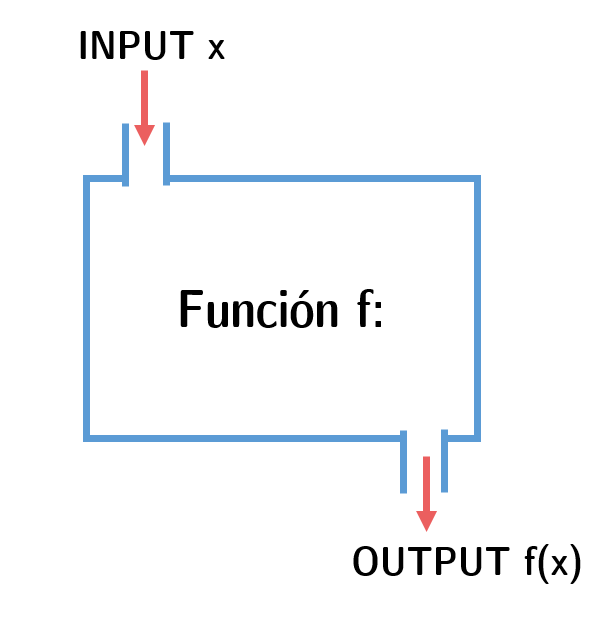
\includegraphics[width=0.8\linewidth]{00-images/fig_3_3}

\texttt{sqrt()} toma un valor numérico como input y devuelve su raíz
cuadrada como output. \texttt{log()} toma el mismo input, pero devuelve
su logaritmo común (o en base a 10). \texttt{c()} toma distintos valores
únicos como input y devuelve un vector que los concatena.

Es a propósito de los vectores que las funciones de R comienzan a
brillar y a alejarse de las cualidades básicas de una calculadora (que,
a grandes rasgos, es lo que hemos visto ahora de R, nada muy
impresionante). Veamos algunas funciones que extraen información útil
sobre nuestro vector. ¿Qué hace cada una?

\begin{Shaded}
\begin{Highlighting}[]
\KeywordTok{mean}\NormalTok{(vector_}\DecValTok{1}\NormalTok{) }\CommentTok{# media}
\end{Highlighting}
\end{Shaded}

\begin{verbatim}
## [1] 15
\end{verbatim}

\begin{Shaded}
\begin{Highlighting}[]
\KeywordTok{median}\NormalTok{(vector_}\DecValTok{1}\NormalTok{) }\CommentTok{# mediana}
\end{Highlighting}
\end{Shaded}

\begin{verbatim}
## [1] 15
\end{verbatim}

\begin{Shaded}
\begin{Highlighting}[]
\KeywordTok{sd}\NormalTok{(vector_}\DecValTok{1}\NormalTok{) }\CommentTok{# desviación estándar}
\end{Highlighting}
\end{Shaded}

\begin{verbatim}
## [1] 5
\end{verbatim}

\begin{Shaded}
\begin{Highlighting}[]
\KeywordTok{sum}\NormalTok{(vector_}\DecValTok{1}\NormalTok{) }\CommentTok{# suma}
\end{Highlighting}
\end{Shaded}

\begin{verbatim}
## [1] 45
\end{verbatim}

\begin{Shaded}
\begin{Highlighting}[]
\KeywordTok{min}\NormalTok{(vector_}\DecValTok{1}\NormalTok{) }\CommentTok{# valor mínimo}
\end{Highlighting}
\end{Shaded}

\begin{verbatim}
## [1] 10
\end{verbatim}

\begin{Shaded}
\begin{Highlighting}[]
\KeywordTok{max}\NormalTok{(vector_}\DecValTok{1}\NormalTok{) }\CommentTok{# valor máximo}
\end{Highlighting}
\end{Shaded}

\begin{verbatim}
## [1] 20
\end{verbatim}

\begin{Shaded}
\begin{Highlighting}[]
\KeywordTok{length}\NormalTok{(vector_}\DecValTok{1}\NormalTok{) }\CommentTok{# longitud (cantidad de valores)}
\end{Highlighting}
\end{Shaded}

\begin{verbatim}
## [1] 3
\end{verbatim}

\begin{Shaded}
\begin{Highlighting}[]
\KeywordTok{sort}\NormalTok{(vector_}\DecValTok{1}\NormalTok{) }\CommentTok{# ...}
\end{Highlighting}
\end{Shaded}

\begin{verbatim}
## [1] 10 15 20
\end{verbatim}

El lector podría haber deducido que \texttt{sort()}, la última función
del lote anterior, ordena al vector de menor a mayor. ¿Qué pasa si
quisiéramos ordenarlo de mayor a menor? Esto nos permite introducir a
los \emph{argumentos}, partes de las funciones que nos permiten
modificar su comportamiento. A continuación agregaremos el argumento
\texttt{decreasing\ =\ TRUE} al comando anterior, consiguiendo nuestro
objetivo:

\begin{Shaded}
\begin{Highlighting}[]
\KeywordTok{sort}\NormalTok{(vector_}\DecValTok{1}\NormalTok{, }\DataTypeTok{decreasing =} \OtherTok{TRUE}\NormalTok{)}
\end{Highlighting}
\end{Shaded}

\begin{verbatim}
## [1] 20 15 10
\end{verbatim}

\subsection{Archivos / gráficos / paquetes /
ayuda}\label{archivos-graficos-paquetes-ayuda}

El panel inferior derecho de RStudio. Estas cuatro pestañas son las que
se roban la película.

\subsubsection{Archivos}\label{archivos}

Esta pestaña es una ventana a nuestros archivos. Funcionando como un
pequeño gestor, nos permite moverlos, renombrarlos, copiarlos, etcétera.
A propósito de archivos, una de las grandes novedades recientes de R son
los \emph{RStudio Projects}, o proyectos de RStudio. Los desarrolladores
de RStudio se dieron cuenta de que sus usuarios tenían scripts y otros
archivos de R (de los que aprenderemos luego, como bases de datos)
desperdigados a lo largo y ancho de sus discos duros, sin orden alguno.
Por eso implementaron la filosofía de ``un proyecto, una carpeta''. Es
tan simple como suena: la idea es que cada proyecto en el que trabajemos
sea autosuficiente, que incluya todo lo que necesitemos en una sola
carpeta. Se pueden manejar los proyectos desde la esquina superior
derecha de R. El lector debe ser cuidadoso y notar que crear o abrir un
proyecto reiniciará su sesión de R, borrando todo el trabajo que no
guarde.

\emph{screenshot de RStudio Projects}

\subsubsection{Gráficos}\label{graficos}

Aquí aparecen los gráficos que realizamos con R. ¡En el capítulo
\emph{X} aprenderemos a crearlos!

\subsubsection{Paquetes}\label{paquetes}

Una de las cualidades de R a la que más hincapié hemos dado es su
versatilidad. Su código libre hace que muchos desarrolladores se sientan
atraídos a aportar a la comunidad de R con nuevas funcionalidades. En
general, realizan esto a través de paquetes, que los usuarios pueden
instalar como apéndices adicionales a R. Los paquetes contienen nuevas
funciones, bases de datos, etcétera. La pestaña de RStudio aquí reseñada
nos permite acceder a nuestros paquetes instalados.

Instalar un paquete es bastante simple, a través de la función
\texttt{install.packages()}. A continuación vamos a instalar el paquete
``tidyverse'', central en nuestros próximos análisis. El tidyverse es
una recopilación que incluye algunos de los mejores paquetes modernos
para análisis de datos en R.

\begin{Shaded}
\begin{Highlighting}[]
\KeywordTok{install.packages}\NormalTok{(}\StringTok{"tidyverse"}\NormalTok{)}
\end{Highlighting}
\end{Shaded}

Cada vez que el usuario abre una nueva sesión de R, este carga ``como de
fábrica''. No solo sin objetos, sino que solo con los paquetes nucleares
que permiten a R funcionar. Tenemos que cargar los paquetes extra que
queramos usar, entonces. La forma más común de hacer esto es a través de
la función \texttt{library()}, como se ve a continuación:

\begin{Shaded}
\begin{Highlighting}[]
\KeywordTok{library}\NormalTok{(}\StringTok{"tidyverse"}\NormalTok{)}
\end{Highlighting}
\end{Shaded}

\begin{verbatim}
## Warning: package 'tidyverse' was built under R version 3.4.1
\end{verbatim}

\begin{verbatim}
## Loading tidyverse: ggplot2
## Loading tidyverse: tibble
## Loading tidyverse: tidyr
## Loading tidyverse: readr
## Loading tidyverse: purrr
## Loading tidyverse: dplyr
\end{verbatim}

\begin{verbatim}
## Warning: package 'tibble' was built under R version 3.4.1
\end{verbatim}

\begin{verbatim}
## Warning: package 'dplyr' was built under R version 3.4.1
\end{verbatim}

\begin{verbatim}
## Conflicts with tidy packages ----------------------------------------------
\end{verbatim}

\begin{verbatim}
## filter(): dplyr, stats
## lag():    dplyr, stats
\end{verbatim}

El lector puede ahorrarse el trabajo de instalar los paquetes utilizados
en \emph{analizaR datos políticos} en el futuro y hacerlo todo ahora,
corriendo el siguiente súper comando. Ojo: ¡esto no lo salvará de cargar
los paquetes en cada nueva sesión de R que inicie! Ojo 2: puede que esto
le tome un tiempo considerable.

\emph{paquetes a instalar}

\subsubsection{Ayuda}\label{ayuda}

Buscar ayuda es central a la hora de programar (y no solo de
programar\ldots{}). Esta pestaña de RStudio abre los archivos de ayuda
que necesitemos, permitiéndonos buscar en ellos. Las funciones tienen
archivos de ayuda para sí solas. Por ejemplo, podemos acceder al archivo
de ayuda de la función \texttt{sqrt()} a través del comando
\texttt{help(sqrt)}. Los paquetes en su conjunto también tienen archivos
de ayuda, más comprensivos. Por ejemplo, para ver los archivos de ayuda
del tidyverse solo debemos recurrir al argumento ``package'':
\texttt{help(package\ =\ tidyverse)}. El lector debe notar que los
archivos de ayuda de paquetes y funciones de paquetes solo están
disponibles si el paquete ha sido cargado.

\section{Ejercicios}\label{ejercicios}

\begin{itemize}
\tightlist
\item
  ¿Qué significa ``correr'' un comando desde un script? ¿Cómo se hace?
\item
  ¿Cuál es la media de los dígitos del hit de Rafaella Carrà, 0 3 0 3 4
  5 6? ¿Y la mediana? Por último, órdenelos de mayor a menor.
\item
  Busque ayuda para el paquete ``googledrive''. Recomendado:
  maravillarse con la variedad de los paquetes de R.
\end{itemize}

\chapter{Manejo}\label{manejo}

Cuando hablamos de análisis de datos, casi siempre nos referimos a
análisis de \emph{bases de datos}. Aunque hay varios formatos de bases
de datos disponibles, en ciencias sociales generalmente usamos y creamos
\emph{bases de datos tabulares}, que son las que este libro tratará. Muy
probablemente el lector estará familiarizado con la estructura básica de
este tipo de bases, gracias a las planillas de Microsoft Excel, Google
Spreadsheets y/o LibreOffice Calc. La primera fila suele ser un
\textbf{header} o encabezado, que indica qué datos registran las celdas
de esa columna. En general, queremos que nuestras bases de datos
tabulares tengan una estructura \emph{tidy}, como la siguiente:

\includegraphics{http://garrettgman.github.io/images/tidy-4.png}
(traducir!)

La idea es simple: cada columna es una variable, cada fila una
observación (de acuerdo a la unidad de análisis) y, por lo tanto, cada
celda es una observación.

\section{Nuestra base de datos}\label{nuestra-base-de-datos}

Para este capítulo usaremos una sección de la base de datos de Quality
of Government (QoG, 2017), un proyecto que registra diversos datos de
países. Sus primeras observaciones son las siguientes:

\begin{verbatim}
## Warning: package 'bindrcpp' was built under R version 3.4.1
\end{verbatim}

\begin{tabular}{l|r|r|r|r|r|l}
\hline
cname & wdi\_gdppppcon2011 & wdi\_pop & ti\_cpi & lp\_muslim80 & fh\_ipolity2 & region\\
\hline
Afghanistan & 57566228480 & 30682500 & 8 & 99.3 & 2.018881 & Southern Asia\\
\hline
Albania & 28715335680 & 2897366 & 31 & 20.5 & 8.083333 & Southern Europe\\
\hline
Algeria & 507901640704 & 38186136 & 36 & 99.1 & 4.250000 & Northern Africa\\
\hline
Angola & 152477499392 & 23448202 & 23 & 0.0 & 3.250000 & Middle Africa\\
\hline
Australia & 990474338304 & 23125868 & 81 & 0.2 & 10.000000 & Australia and New Zealand\\
\hline
Austria & 373413642240 & 8479375 & 69 & 0.6 & 10.000000 & Western Europe\\
\hline
\end{tabular}

Las variables son las siguientes:

\begin{longtable}[]{@{}ll@{}}
\toprule
\begin{minipage}[b]{0.16\columnwidth}\raggedright\strut
variable\strut
\end{minipage} & \begin{minipage}[b]{0.78\columnwidth}\raggedright\strut
descripción\strut
\end{minipage}\tabularnewline
\midrule
\endhead
\begin{minipage}[t]{0.16\columnwidth}\raggedright\strut
cname\strut
\end{minipage} & \begin{minipage}[t]{0.78\columnwidth}\raggedright\strut
Nombre del país\strut
\end{minipage}\tabularnewline
\begin{minipage}[t]{0.16\columnwidth}\raggedright\strut
wdi\_gdppppcon2011\strut
\end{minipage} & \begin{minipage}[t]{0.78\columnwidth}\raggedright\strut
GDP PPP, en dólares del 2011, según los datos de WDI (p.~635 del
codebook)\strut
\end{minipage}\tabularnewline
\begin{minipage}[t]{0.16\columnwidth}\raggedright\strut
wdi\_pop\strut
\end{minipage} & \begin{minipage}[t]{0.78\columnwidth}\raggedright\strut
Población, según los datos de WDI (p.~665)\strut
\end{minipage}\tabularnewline
\begin{minipage}[t]{0.16\columnwidth}\raggedright\strut
ti\_cpi\strut
\end{minipage} & \begin{minipage}[t]{0.78\columnwidth}\raggedright\strut
Índice de Percepción de la Corrupción de TI. Va de 0 a 100, con 0 lo más
corrupto (p.~560)\strut
\end{minipage}\tabularnewline
\begin{minipage}[t]{0.16\columnwidth}\raggedright\strut
lp\_muslim80\strut
\end{minipage} & \begin{minipage}[t]{0.78\columnwidth}\raggedright\strut
Porcentaje de población de religión musulmana, para 1980, según LP
(p.~447)\strut
\end{minipage}\tabularnewline
\begin{minipage}[t]{0.16\columnwidth}\raggedright\strut
fh\_ipolity2\strut
\end{minipage} & \begin{minipage}[t]{0.78\columnwidth}\raggedright\strut
Nivel de democracia según FH. Va de 0 a 10, con 0 como menos democrático
(p.~291)\strut
\end{minipage}\tabularnewline
\begin{minipage}[t]{0.16\columnwidth}\raggedright\strut
region\strut
\end{minipage} & \begin{minipage}[t]{0.78\columnwidth}\raggedright\strut
Región del país, según WDI (añadida a la base)\strut
\end{minipage}\tabularnewline
\bottomrule
\end{longtable}

Para comenzar a trabajar carguemos el paquete tidyverse, uno de los
centrales del libro, que nos dará funciones útiles para trabajar con
nuestra base datos.

\begin{Shaded}
\begin{Highlighting}[]
\KeywordTok{library}\NormalTok{(}\StringTok{"tidyverse"}\NormalTok{)}
\end{Highlighting}
\end{Shaded}

Ahora carguemos la base de datos a nuestro ambiente de trabajo en R.
Vamos a llamarla ``qog\_mod'' (QoG modificada). El archivo está en
formato .csv, por lo que utilizaremos la función del tidyverse
\texttt{read\_csv()}

\begin{Shaded}
\begin{Highlighting}[]
\NormalTok{qog_mod <-}\StringTok{ }\KeywordTok{read_csv}\NormalTok{(}\StringTok{"00-datos/04_qog_mod.csv"}\NormalTok{)}
\end{Highlighting}
\end{Shaded}

\begin{verbatim}
## Parsed with column specification:
## cols(
##   cname = col_character(),
##   wdi_gdppppcon2011 = col_double(),
##   wdi_pop = col_integer(),
##   ti_cpi = col_double(),
##   lp_muslim80 = col_double(),
##   fh_ipolity2 = col_double(),
##   region = col_character()
## )
\end{verbatim}

(hay que decidir cómo se va a hacer esto: desde carpeta local, url,
paquete, etc.)

\section{Describir base}\label{describir-base}

(aquí podría ir \texttt{describe\_all()} u otra función de descripción
de la base, habría que decidir si esto tiene sentido en términos
pedagógicos; otra opción es hacer otro capítulo con
\texttt{group\_by()}, \texttt{tabyl()}, \texttt{crosstab()}, etc; me
inclino por esta última opción)

Para aproximarnos a nuestra base recién cargada tenemos varias opciones.
Podemos, como antes, simplemente usar su nombre como un comando para un
resumen rápido:

\begin{Shaded}
\begin{Highlighting}[]
\NormalTok{qog_mod}
\end{Highlighting}
\end{Shaded}

\begin{verbatim}
## # A tibble: 139 x 7
##          cname wdi_gdppppcon2011   wdi_pop ti_cpi lp_muslim80 fh_ipolity2
##          <chr>             <dbl>     <int>  <dbl>       <dbl>       <dbl>
##  1 Afghanistan       57566228480  30682500      8        99.3   2.0188808
##  2     Albania       28715335680   2897366     31        20.5   8.0833330
##  3     Algeria      507901640704  38186136     36        99.1   4.2500000
##  4      Angola      152477499392  23448202     23         0.0   3.2500000
##  5   Australia      990474338304  23125868     81         0.2  10.0000000
##  6     Austria      373413642240   8479375     69         0.6  10.0000000
##  7     Bahamas        8497731584    377841     71         0.0  10.0000000
##  8     Bahrain       56583507968   1349427     48        95.0   0.8333333
##  9  Bangladesh      446835425280 157157392     27        85.9   6.4166670
## 10    Barbados        4333428224    282503     75         0.2  10.0000000
## # ... with 129 more rows, and 1 more variables: region <chr>
\end{verbatim}

También podemos utilizar la función \texttt{glimpse()} para tener un
resumen desde otra perspectiva:

\begin{Shaded}
\begin{Highlighting}[]
\KeywordTok{glimpse}\NormalTok{(qog_mod)}
\end{Highlighting}
\end{Shaded}

\begin{verbatim}
## Observations: 139
## Variables: 7
## $ cname             <chr> "Afghanistan", "Albania", "Algeria", "Angola...
## $ wdi_gdppppcon2011 <dbl> 5.756623e+10, 2.871534e+10, 5.079016e+11, 1....
## $ wdi_pop           <int> 30682500, 2897366, 38186136, 23448202, 23125...
## $ ti_cpi            <dbl> 8.00000, 31.00000, 36.00000, 23.00000, 81.00...
## $ lp_muslim80       <dbl> 99.3, 20.5, 99.1, 0.0, 0.2, 0.6, 0.0, 95.0, ...
## $ fh_ipolity2       <dbl> 2.0188808, 8.0833330, 4.2500000, 3.2500000, ...
## $ region            <chr> "Southern Asia", "Southern Europe", "Norther...
\end{verbatim}

Una alternativa que nos permite ver la base completa es la función
\texttt{View()}, análoga a clickear nuestro objeto en la pestaña
``Environment'' de Rstudio:

\begin{Shaded}
\begin{Highlighting}[]
\KeywordTok{View}\NormalTok{(qog_mod)}
\end{Highlighting}
\end{Shaded}

\section{Ordenar la base}\label{ordenar-la-base}

Una de las operaciones más comunes con bases de datos es ordenarlas de
acuerdo a alguna de las variables. Esto nos puede dar insights
(¿traducción?) inmediatos sobre nuestras observaciones. Por ejemplo,
ordenemos la base de acuerdo a población:

\begin{Shaded}
\begin{Highlighting}[]
\KeywordTok{arrange}\NormalTok{(qog_mod, wdi_pop)}
\end{Highlighting}
\end{Shaded}

\begin{verbatim}
## # A tibble: 139 x 7
##                    cname wdi_gdppppcon2011 wdi_pop   ti_cpi lp_muslim80
##                    <chr>             <dbl>   <int>    <dbl>       <dbl>
##  1              Dominica         722668736   72005 58.00000         0.0
##  2            Seychelles        2229991168   89900 54.00000         0.3
##  3                 Tonga         513904512  105139 31.39194         0.0
##  4              Kiribati         183852816  108544 30.80074         0.0
##  5              St Lucia        1871906688  182305 71.00000         0.0
##  6 Sao Tome and Principe         540452288  182386 42.00000         0.0
##  7                 Samoa        1047012608  190390 52.00000         0.0
##  8              Barbados        4333428224  282503 75.00000         0.2
##  9               Iceland       13266284544  323764 78.00000         0.0
## 10               Bahamas        8497731584  377841 71.00000         0.0
## # ... with 129 more rows, and 2 more variables: fh_ipolity2 <dbl>,
## #   region <chr>
\end{verbatim}

El lector debe notar cómo el primer argumento, ``qog\_mod'', toma la
base de datos y los siguientes enuncian \textbf{cómo} ordenarla, en este
caso, por ``wdi\_pop'', la variable de población.

Debe notar también cómo el comando anterior no crea ningún objeto, solo
muestra los resultados en la consola. Para crear uno tenemos que seguir
la fórmula típica de asignación:

\begin{Shaded}
\begin{Highlighting}[]
\NormalTok{qog_mod_ordenada <-}\StringTok{ }\KeywordTok{arrange}\NormalTok{(qog_mod, wdi_pop)}
\end{Highlighting}
\end{Shaded}

Podemos realizar ambas operaciones, mostrar los resultados y crear el
objeto, rodeando este último comando con paréntesis:

\begin{Shaded}
\begin{Highlighting}[]
\NormalTok{( qog_mod_ordenada <-}\StringTok{ }\KeywordTok{arrange}\NormalTok{(qog_mod, wdi_pop) )}
\end{Highlighting}
\end{Shaded}

\begin{verbatim}
## # A tibble: 139 x 7
##                    cname wdi_gdppppcon2011 wdi_pop   ti_cpi lp_muslim80
##                    <chr>             <dbl>   <int>    <dbl>       <dbl>
##  1              Dominica         722668736   72005 58.00000         0.0
##  2            Seychelles        2229991168   89900 54.00000         0.3
##  3                 Tonga         513904512  105139 31.39194         0.0
##  4              Kiribati         183852816  108544 30.80074         0.0
##  5              St Lucia        1871906688  182305 71.00000         0.0
##  6 Sao Tome and Principe         540452288  182386 42.00000         0.0
##  7                 Samoa        1047012608  190390 52.00000         0.0
##  8              Barbados        4333428224  282503 75.00000         0.2
##  9               Iceland       13266284544  323764 78.00000         0.0
## 10               Bahamas        8497731584  377841 71.00000         0.0
## # ... with 129 more rows, and 2 more variables: fh_ipolity2 <dbl>,
## #   region <chr>
\end{verbatim}

La operación para ordenar realizada antes iba de menor a mayor, en
términos de población. Si queremos el orden inverso (decreciente), basta
con añadir un signo menos (-) antes de la variable:

\begin{Shaded}
\begin{Highlighting}[]
\KeywordTok{arrange}\NormalTok{(qog_mod, }\OperatorTok{-}\NormalTok{wdi_pop)}
\end{Highlighting}
\end{Shaded}

\begin{verbatim}
## # A tibble: 139 x 7
##               cname wdi_gdppppcon2011    wdi_pop ti_cpi lp_muslim80
##               <chr>             <dbl>      <int>  <dbl>       <dbl>
##  1            China      1.602399e+13 1357379968     40         2.4
##  2            India      6.566166e+12 1279498880     36        11.6
##  3    United States      1.623049e+13  316497536     73         0.8
##  4        Indonesia      2.430922e+12  251268272     32        43.4
##  5           Brazil      3.109302e+12  204259376     42         0.1
##  6 Pakistan (1971-)      8.109545e+11  181192640     28        96.8
##  7          Nigeria      9.414628e+11  172816512     25        45.0
##  8       Bangladesh      4.468354e+11  157157392     27        85.9
##  9            Japan      4.535077e+12  127338624     74         0.0
## 10           Mexico      1.997247e+12  123740112     34         0.0
## # ... with 129 more rows, and 2 more variables: fh_ipolity2 <dbl>,
## #   region <chr>
\end{verbatim}

¡Con eso tenemos los países con mayor población en el mundo! ¿Qué pasa
si queremos los países con mayor población \textbf{dentro de cada
región}? Tendríamos que realizar un ordenamiento en dos pasos: primero
por región y luego por población. Con \texttt{arrange()} esto es simple:

\begin{Shaded}
\begin{Highlighting}[]
\KeywordTok{arrange}\NormalTok{(qog_mod, region, }\OperatorTok{-}\NormalTok{wdi_pop)}
\end{Highlighting}
\end{Shaded}

\begin{verbatim}
## # A tibble: 139 x 7
##                  cname wdi_gdppppcon2011  wdi_pop ti_cpi lp_muslim80
##                  <chr>             <dbl>    <int>  <dbl>       <dbl>
##  1           Australia      990474338304 23125868     81         0.2
##  2         New Zealand      148189986816  4442100     91         0.0
##  3                Cuba      226685157376 11362505     46         0.0
##  4               Haiti       16999370752 10431249     19         0.0
##  5  Dominican Republic      122657308672 10281408     29         0.0
##  6             Jamaica       22884503552  2714734     38         0.1
##  7 Trinidad and Tobago       40973463552  1348240     38         6.5
##  8             Bahamas        8497731584   377841     71         0.0
##  9            Barbados        4333428224   282503     75         0.2
## 10            St Lucia        1871906688   182305     71         0.0
## # ... with 129 more rows, and 2 more variables: fh_ipolity2 <dbl>,
## #   region <chr>
\end{verbatim}

A propósito del resultado anterior, el lector puede deducir que cuando
\texttt{arrange()} ordena variables categóricas (en vez de numéricas) lo
hace alfabéticamente. Añadir un signo menos (-) antes de la variable
hará que el orden sea al revés en términos del alfabeto:

\begin{Shaded}
\begin{Highlighting}[]
\KeywordTok{arrange}\NormalTok{(qog_mod, }\KeywordTok{desc}\NormalTok{(region), }\OperatorTok{-}\NormalTok{wdi_pop) }\CommentTok{# no sé por qué - no funciona, ARREGLAR}
\end{Highlighting}
\end{Shaded}

\begin{verbatim}
## # A tibble: 139 x 7
##                   cname wdi_gdppppcon2011  wdi_pop ti_cpi lp_muslim80
##                   <chr>             <dbl>    <int>  <dbl>       <dbl>
##  1       France (1963-)      2.459435e+12 65925496     71         3.0
##  2          Netherlands      7.623825e+11 16804432     83         1.0
##  3              Belgium      4.521544e+11 11182817     75         1.1
##  4              Austria      3.734136e+11  8479375     69         0.6
##  5          Switzerland      4.442016e+11  8089346     85         0.3
##  6           Luxembourg      4.884228e+10   543360     80         0.0
##  7               Turkey      1.392197e+12 75010200     50        99.2
##  8                 Iraq      5.108955e+11 33781384     16        95.8
##  9         Saudi Arabia      1.478748e+12 30201052     46        98.8
## 10 United Arab Emirates      5.609863e+11  9039978     69        94.9
## # ... with 129 more rows, and 2 more variables: fh_ipolity2 <dbl>,
## #   region <chr>
\end{verbatim}

\section{Seleccionar columnas}\label{seleccionar-columnas}

A veces queremos trabajar solo con algunas variables de una base de
datos. Para esto existe la función \texttt{select()}. Pensemos que
queremos solo el nombre de cada país (cname) y su porcentaje de
población musulmana para 1980:

\begin{Shaded}
\begin{Highlighting}[]
\KeywordTok{select}\NormalTok{(qog_mod, cname, lp_muslim80)}
\end{Highlighting}
\end{Shaded}

\begin{verbatim}
## # A tibble: 139 x 2
##          cname lp_muslim80
##          <chr>       <dbl>
##  1 Afghanistan        99.3
##  2     Albania        20.5
##  3     Algeria        99.1
##  4      Angola         0.0
##  5   Australia         0.2
##  6     Austria         0.6
##  7     Bahamas         0.0
##  8     Bahrain        95.0
##  9  Bangladesh        85.9
## 10    Barbados         0.2
## # ... with 129 more rows
\end{verbatim}

Al igual que para \texttt{arrange()}, aquí el primer argumento designa
la base a modificar y los demás cómo se debería hacer eso -en este caso,
qué variables deben ser seleccionadas.

Añadir un signo menos (-) aquí indica qué variables \emph{no}
seleccionar. Por ejemplo, quitemos el porcentaje de población musulmana
para 1980 de la base:

\begin{Shaded}
\begin{Highlighting}[]
\KeywordTok{select}\NormalTok{(qog_mod, }\OperatorTok{-}\NormalTok{lp_muslim80)}
\end{Highlighting}
\end{Shaded}

\begin{verbatim}
## # A tibble: 139 x 6
##          cname wdi_gdppppcon2011   wdi_pop ti_cpi fh_ipolity2
##          <chr>             <dbl>     <int>  <dbl>       <dbl>
##  1 Afghanistan       57566228480  30682500      8   2.0188808
##  2     Albania       28715335680   2897366     31   8.0833330
##  3     Algeria      507901640704  38186136     36   4.2500000
##  4      Angola      152477499392  23448202     23   3.2500000
##  5   Australia      990474338304  23125868     81  10.0000000
##  6     Austria      373413642240   8479375     69  10.0000000
##  7     Bahamas        8497731584    377841     71  10.0000000
##  8     Bahrain       56583507968   1349427     48   0.8333333
##  9  Bangladesh      446835425280 157157392     27   6.4166670
## 10    Barbados        4333428224    282503     75  10.0000000
## # ... with 129 more rows, and 1 more variables: region <chr>
\end{verbatim}

Aparte de seleccionar variables específicas, \texttt{select()} es capaz
de entender referencias a intervalos de variables. Por ejemplo, podemos
querer las cuatro primeras variables:

\begin{Shaded}
\begin{Highlighting}[]
\KeywordTok{select}\NormalTok{(qog_mod, cname}\OperatorTok{:}\NormalTok{ti_cpi)}
\end{Highlighting}
\end{Shaded}

\begin{verbatim}
## # A tibble: 139 x 4
##          cname wdi_gdppppcon2011   wdi_pop ti_cpi
##          <chr>             <dbl>     <int>  <dbl>
##  1 Afghanistan       57566228480  30682500      8
##  2     Albania       28715335680   2897366     31
##  3     Algeria      507901640704  38186136     36
##  4      Angola      152477499392  23448202     23
##  5   Australia      990474338304  23125868     81
##  6     Austria      373413642240   8479375     69
##  7     Bahamas        8497731584    377841     71
##  8     Bahrain       56583507968   1349427     48
##  9  Bangladesh      446835425280 157157392     27
## 10    Barbados        4333428224    282503     75
## # ... with 129 more rows
\end{verbatim}

\begin{Shaded}
\begin{Highlighting}[]
\KeywordTok{select}\NormalTok{(qog_mod, }\DecValTok{1}\OperatorTok{:}\DecValTok{4}\NormalTok{) }\CommentTok{# lo mismo, aunque no recomendado}
\end{Highlighting}
\end{Shaded}

\begin{verbatim}
## # A tibble: 139 x 4
##          cname wdi_gdppppcon2011   wdi_pop ti_cpi
##          <chr>             <dbl>     <int>  <dbl>
##  1 Afghanistan       57566228480  30682500      8
##  2     Albania       28715335680   2897366     31
##  3     Algeria      507901640704  38186136     36
##  4      Angola      152477499392  23448202     23
##  5   Australia      990474338304  23125868     81
##  6     Austria      373413642240   8479375     69
##  7     Bahamas        8497731584    377841     71
##  8     Bahrain       56583507968   1349427     48
##  9  Bangladesh      446835425280 157157392     27
## 10    Barbados        4333428224    282503     75
## # ... with 129 more rows
\end{verbatim}

Otra herramienta para complejizar nuestra selección se encuentra en las
funciones de ayuda. Entre ellas, \texttt{starts\_with} es de particular
utilidad, permitiendo seleccionar variables que empiecen con cierto
patrón. Por ejemplo, podríamos querer, a partir del nombre del país,
todas las variables que provengan de los World Development Indicators
(WDI) del Banco Mundial:

\begin{Shaded}
\begin{Highlighting}[]
\KeywordTok{select}\NormalTok{(qog_mod, cname, }\KeywordTok{starts_with}\NormalTok{(}\StringTok{"wdi_"}\NormalTok{))}
\end{Highlighting}
\end{Shaded}

\begin{verbatim}
## # A tibble: 139 x 3
##          cname wdi_gdppppcon2011   wdi_pop
##          <chr>             <dbl>     <int>
##  1 Afghanistan       57566228480  30682500
##  2     Albania       28715335680   2897366
##  3     Algeria      507901640704  38186136
##  4      Angola      152477499392  23448202
##  5   Australia      990474338304  23125868
##  6     Austria      373413642240   8479375
##  7     Bahamas        8497731584    377841
##  8     Bahrain       56583507968   1349427
##  9  Bangladesh      446835425280 157157392
## 10    Barbados        4333428224    282503
## # ... with 129 more rows
\end{verbatim}

Otra función de ayuda útil es \texttt{everything()}, que se lee como
``todas las demás variables''. Es especialmente útil para cambiar el
orden de las variables en una bases de datos. Por ejemplo, pasemos
región al segundo lugar entre las variables:

\begin{Shaded}
\begin{Highlighting}[]
\KeywordTok{select}\NormalTok{(qog_mod, cname, region, }\KeywordTok{everything}\NormalTok{())}
\end{Highlighting}
\end{Shaded}

\begin{verbatim}
## # A tibble: 139 x 7
##          cname                    region wdi_gdppppcon2011   wdi_pop
##          <chr>                     <chr>             <dbl>     <int>
##  1 Afghanistan             Southern Asia       57566228480  30682500
##  2     Albania           Southern Europe       28715335680   2897366
##  3     Algeria           Northern Africa      507901640704  38186136
##  4      Angola             Middle Africa      152477499392  23448202
##  5   Australia Australia and New Zealand      990474338304  23125868
##  6     Austria            Western Europe      373413642240   8479375
##  7     Bahamas                 Caribbean        8497731584    377841
##  8     Bahrain              Western Asia       56583507968   1349427
##  9  Bangladesh             Southern Asia      446835425280 157157392
## 10    Barbados                 Caribbean        4333428224    282503
## # ... with 129 more rows, and 3 more variables: ti_cpi <dbl>,
## #   lp_muslim80 <dbl>, fh_ipolity2 <dbl>
\end{verbatim}

\section{Renombrar columnas}\label{renombrar-columnas}

La notación para el GDP es un poco confusa. ¿Y si queremos cambiar el
nombre de la variable? Aprovechemos también de cambiar el nombre de la
variable de identificación por país.

\begin{Shaded}
\begin{Highlighting}[]
\KeywordTok{rename}\NormalTok{(qog_mod, }\DataTypeTok{wdi_gdp =}\NormalTok{ wdi_gdppppcon2011, }\DataTypeTok{country_name =}\NormalTok{ cname)}
\end{Highlighting}
\end{Shaded}

\begin{verbatim}
## # A tibble: 139 x 7
##    country_name      wdi_gdp   wdi_pop ti_cpi lp_muslim80 fh_ipolity2
##           <chr>        <dbl>     <int>  <dbl>       <dbl>       <dbl>
##  1  Afghanistan  57566228480  30682500      8        99.3   2.0188808
##  2      Albania  28715335680   2897366     31        20.5   8.0833330
##  3      Algeria 507901640704  38186136     36        99.1   4.2500000
##  4       Angola 152477499392  23448202     23         0.0   3.2500000
##  5    Australia 990474338304  23125868     81         0.2  10.0000000
##  6      Austria 373413642240   8479375     69         0.6  10.0000000
##  7      Bahamas   8497731584    377841     71         0.0  10.0000000
##  8      Bahrain  56583507968   1349427     48        95.0   0.8333333
##  9   Bangladesh 446835425280 157157392     27        85.9   6.4166670
## 10     Barbados   4333428224    282503     75         0.2  10.0000000
## # ... with 129 more rows, and 1 more variables: region <chr>
\end{verbatim}

\section{Filtrar observaciones}\label{filtrar-observaciones}

Es muy común el querer filtrar nuestras observaciones de acuerdo a algún
tipo de criterio lógico. Para esto R cuenta con operadores lógicos. Los
más comunes son los siguientes:

\begin{longtable}[]{@{}cl@{}}
\toprule
operador & descripción\tabularnewline
\midrule
\endhead
== & es igual a\tabularnewline
!= & es distinto a\tabularnewline
\textgreater{} & es mayor a\tabularnewline
\textless{} & es menor a\tabularnewline
\textgreater{}= & es mayor o igual a\tabularnewline
\textless{}= & es menor o igual a\tabularnewline
\& & y (intersección)\tabularnewline
&\tabularnewline
\bottomrule
\end{longtable}

Por ejemplo, podríamos querer solo los países (observaciones)
sudamericanos. Hacer esto con \texttt{filter()} es simple, con la ayuda
de operadores lógicos:

\begin{Shaded}
\begin{Highlighting}[]
\KeywordTok{filter}\NormalTok{(qog_mod, region }\OperatorTok{==}\StringTok{ "South America"}\NormalTok{)}
\end{Highlighting}
\end{Shaded}

\begin{verbatim}
## # A tibble: 11 x 7
##        cname wdi_gdppppcon2011   wdi_pop ti_cpi lp_muslim80 fh_ipolity2
##        <chr>             <dbl>     <int>  <dbl>       <dbl>       <dbl>
##  1   Bolivia      6.334484e+10  10399931     34         0.0    7.583333
##  2    Brazil      3.109302e+12 204259376     42         0.1    8.666666
##  3     Chile      3.831625e+11  17575832     71         0.0   10.000000
##  4  Colombia      5.824887e+11  47342364     36         0.2    7.166667
##  5   Ecuador      1.664122e+11  15661312     35         0.0    7.083333
##  6    Guyana      5.066298e+09    761033     27         9.0    7.750000
##  7  Paraguay      5.319503e+10   6465669     24         0.0    8.083333
##  8      Peru      3.461269e+11  30565460     38         0.0    8.500000
##  9  Suriname      8.388805e+09    533450     36        13.0    7.916666
## 10   Uruguay      6.582768e+10   3407969     73         0.0   10.000000
## 11 Venezuela      5.355721e+11  30276044     20         0.0    5.166666
## # ... with 1 more variables: region <chr>
\end{verbatim}

¿Qué pasa si queremos solo las filas de países sudamericanos con más de
10 millones de habitantes (nos quedamos con 8 de 12)?

¿Cuáles son los filtros que aplican los siguientes comandos?

\begin{Shaded}
\begin{Highlighting}[]
\KeywordTok{filter}\NormalTok{(qog_mod, fh_ipolity2 }\OperatorTok{>}\StringTok{ }\DecValTok{9}\NormalTok{)}
\end{Highlighting}
\end{Shaded}

\begin{verbatim}
## # A tibble: 39 x 7
##             cname wdi_gdppppcon2011  wdi_pop ti_cpi lp_muslim80
##             <chr>             <dbl>    <int>  <dbl>       <dbl>
##  1      Australia      9.904743e+11 23125868     81         0.2
##  2        Austria      3.734136e+11  8479375     69         0.6
##  3        Bahamas      8.497732e+09   377841     71         0.0
##  4       Barbados      4.333428e+09   282503     75         0.2
##  5        Belgium      4.521544e+11 11182817     75         1.1
##  6         Canada      1.484142e+12 35158304     81         0.6
##  7     Cape Verde      3.109325e+09   507258     58         0.0
##  8          Chile      3.831625e+11 17575832     71         0.0
##  9     Costa Rica      6.541985e+10  4706433     53         0.0
## 10 Cyprus (1975-)      2.592799e+10  1141652     63        18.5
## # ... with 29 more rows, and 2 more variables: fh_ipolity2 <dbl>,
## #   region <chr>
\end{verbatim}

\begin{Shaded}
\begin{Highlighting}[]
\KeywordTok{filter}\NormalTok{(qog_mod, wdi_pop }\OperatorTok{>}\StringTok{ }\FloatTok{10e7}\NormalTok{)}
\end{Highlighting}
\end{Shaded}

\begin{verbatim}
## # A tibble: 10 x 7
##               cname wdi_gdppppcon2011    wdi_pop ti_cpi lp_muslim80
##               <chr>             <dbl>      <int>  <dbl>       <dbl>
##  1       Bangladesh      4.468354e+11  157157392     27        85.9
##  2           Brazil      3.109302e+12  204259376     42         0.1
##  3            China      1.602399e+13 1357379968     40         2.4
##  4            India      6.566166e+12 1279498880     36        11.6
##  5        Indonesia      2.430922e+12  251268272     32        43.4
##  6            Japan      4.535077e+12  127338624     74         0.0
##  7           Mexico      1.997247e+12  123740112     34         0.0
##  8          Nigeria      9.414628e+11  172816512     25        45.0
##  9 Pakistan (1971-)      8.109545e+11  181192640     28        96.8
## 10    United States      1.623049e+13  316497536     73         0.8
## # ... with 2 more variables: fh_ipolity2 <dbl>, region <chr>
\end{verbatim}

\begin{Shaded}
\begin{Highlighting}[]
\KeywordTok{filter}\NormalTok{(qog_mod, cname }\OperatorTok{!=}\StringTok{ "Albania"}\NormalTok{)}
\end{Highlighting}
\end{Shaded}

\begin{verbatim}
## # A tibble: 138 x 7
##          cname wdi_gdppppcon2011   wdi_pop ti_cpi lp_muslim80 fh_ipolity2
##          <chr>             <dbl>     <int>  <dbl>       <dbl>       <dbl>
##  1 Afghanistan       57566228480  30682500      8        99.3   2.0188808
##  2     Algeria      507901640704  38186136     36        99.1   4.2500000
##  3      Angola      152477499392  23448202     23         0.0   3.2500000
##  4   Australia      990474338304  23125868     81         0.2  10.0000000
##  5     Austria      373413642240   8479375     69         0.6  10.0000000
##  6     Bahamas        8497731584    377841     71         0.0  10.0000000
##  7     Bahrain       56583507968   1349427     48        95.0   0.8333333
##  8  Bangladesh      446835425280 157157392     27        85.9   6.4166670
##  9    Barbados        4333428224    282503     75         0.2  10.0000000
## 10     Belgium      452154359808  11182817     75         1.1   9.5000000
## # ... with 128 more rows, and 1 more variables: region <chr>
\end{verbatim}

\begin{Shaded}
\begin{Highlighting}[]
\KeywordTok{filter}\NormalTok{(qog_mod, lp_muslim80 }\OperatorTok{>=}\StringTok{ }\DecValTok{95}\NormalTok{)}
\end{Highlighting}
\end{Shaded}

\begin{verbatim}
## # A tibble: 15 x 7
##               cname wdi_gdppppcon2011   wdi_pop   ti_cpi lp_muslim80
##               <chr>             <dbl>     <int>    <dbl>       <dbl>
##  1      Afghanistan      5.756623e+10  30682500  8.00000        99.3
##  2          Algeria      5.079016e+11  38186136 36.00000        99.1
##  3          Bahrain      5.658351e+10   1349427 48.00000        95.0
##  4             Iran      1.236225e+12  77152448 25.00000        97.9
##  5             Iraq      5.108955e+11  33781384 16.00000        95.8
##  6           Kuwait      2.665846e+11   3593689 43.00000        95.1
##  7            Libya      1.225442e+11   6265987 15.00000        98.1
##  8         Maldives      4.501654e+09    393000 24.70782        99.9
##  9       Mauritania      1.392070e+10   3872684 30.00000        99.4
## 10          Morocco      2.406042e+11  33452686 37.00000        99.4
## 11             Oman      1.517266e+11   3906912 47.00000        98.9
## 12 Pakistan (1971-)      8.109545e+11 181192640 28.00000        96.8
## 13     Saudi Arabia      1.478748e+12  30201052 46.00000        98.8
## 14          Tunisia      1.168218e+11  10886500 41.00000        99.4
## 15           Turkey      1.392197e+12  75010200 50.00000        99.2
## # ... with 2 more variables: fh_ipolity2 <dbl>, region <chr>
\end{verbatim}

\begin{Shaded}
\begin{Highlighting}[]
\KeywordTok{filter}\NormalTok{(qog_mod, region }\OperatorTok{==}\StringTok{ "South America"} \OperatorTok{&}\StringTok{ }\NormalTok{wdi_pop }\OperatorTok{>}\StringTok{ }\FloatTok{10e6}\NormalTok{)}
\end{Highlighting}
\end{Shaded}

\begin{verbatim}
## # A tibble: 7 x 7
##       cname wdi_gdppppcon2011   wdi_pop ti_cpi lp_muslim80 fh_ipolity2
##       <chr>             <dbl>     <int>  <dbl>       <dbl>       <dbl>
## 1   Bolivia      6.334484e+10  10399931     34         0.0    7.583333
## 2    Brazil      3.109302e+12 204259376     42         0.1    8.666666
## 3     Chile      3.831625e+11  17575832     71         0.0   10.000000
## 4  Colombia      5.824887e+11  47342364     36         0.2    7.166667
## 5   Ecuador      1.664122e+11  15661312     35         0.0    7.083333
## 6      Peru      3.461269e+11  30565460     38         0.0    8.500000
## 7 Venezuela      5.355721e+11  30276044     20         0.0    5.166666
## # ... with 1 more variables: region <chr>
\end{verbatim}

\begin{Shaded}
\begin{Highlighting}[]
\KeywordTok{filter}\NormalTok{(qog_mod, region }\OperatorTok{==}\StringTok{ "South America"} \OperatorTok{|}\StringTok{ }\NormalTok{region }\OperatorTok{==}\StringTok{ "South-Eastern Asia"}\NormalTok{)}
\end{Highlighting}
\end{Shaded}

\begin{verbatim}
## # A tibble: 19 x 7
##               cname wdi_gdppppcon2011   wdi_pop ti_cpi lp_muslim80
##               <chr>             <dbl>     <int>  <dbl>       <dbl>
##  1          Bolivia      6.334484e+10  10399931     34         0.0
##  2           Brazil      3.109302e+12 204259376     42         0.1
##  3         Cambodia      4.455977e+10  15078564     20         2.4
##  4            Chile      3.831625e+11  17575832     71         0.0
##  5         Colombia      5.824887e+11  47342364     36         0.2
##  6          Ecuador      1.664122e+11  15661312     35         0.0
##  7           Guyana      5.066298e+09    761033     27         9.0
##  8        Indonesia      2.430922e+12 251268272     32        43.4
##  9             Laos      3.158284e+10   6579985     26         1.0
## 10 Malaysia (1966-)      6.900446e+11  29465372     50        49.4
## 11         Paraguay      5.319503e+10   6465669     24         0.0
## 12             Peru      3.461269e+11  30565460     38         0.0
## 13      Philippines      6.210440e+11  97571680     36         4.3
## 14        Singapore      4.196306e+11   5399200     86        17.4
## 15          Vietnam      4.597249e+11  89708896     31         1.0
## 16         Suriname      8.388805e+09    533450     36        13.0
## 17         Thailand      1.007950e+12  67451424     35         3.9
## 18          Uruguay      6.582768e+10   3407969     73         0.0
## 19        Venezuela      5.355721e+11  30276044     20         0.0
## # ... with 2 more variables: fh_ipolity2 <dbl>, region <chr>
\end{verbatim}

\section{Crear nuevas variables}\label{crear-nuevas-variables}

Muchas veces queremos crear nuevas variables, a partir de las que ya
tenemos. Por ejemplo, podríamos querer el GDP per capita, en vez del
absoluto. Tenemos los ingredientes para calcularlo: el GDP absoluto y la
población. Creemos una nueva variable, entonces:

\begin{Shaded}
\begin{Highlighting}[]
\KeywordTok{mutate}\NormalTok{(qog_mod, }\DataTypeTok{gdp_ppp_per_capita =}\NormalTok{ wdi_gdppppcon2011}\OperatorTok{/}\NormalTok{wdi_pop)}
\end{Highlighting}
\end{Shaded}

\begin{verbatim}
## # A tibble: 139 x 8
##          cname wdi_gdppppcon2011   wdi_pop ti_cpi lp_muslim80 fh_ipolity2
##          <chr>             <dbl>     <int>  <dbl>       <dbl>       <dbl>
##  1 Afghanistan       57566228480  30682500      8        99.3   2.0188808
##  2     Albania       28715335680   2897366     31        20.5   8.0833330
##  3     Algeria      507901640704  38186136     36        99.1   4.2500000
##  4      Angola      152477499392  23448202     23         0.0   3.2500000
##  5   Australia      990474338304  23125868     81         0.2  10.0000000
##  6     Austria      373413642240   8479375     69         0.6  10.0000000
##  7     Bahamas        8497731584    377841     71         0.0  10.0000000
##  8     Bahrain       56583507968   1349427     48        95.0   0.8333333
##  9  Bangladesh      446835425280 157157392     27        85.9   6.4166670
## 10    Barbados        4333428224    282503     75         0.2  10.0000000
## # ... with 129 more rows, and 2 more variables: region <chr>,
## #   gdp_ppp_per_capita <dbl>
\end{verbatim}

Otra nueva variable que podría interesarnos es el número de musulmanes
por país. Con la proporción de musulmanes y la población total del país
podemos hacer una buena estimación:

\begin{Shaded}
\begin{Highlighting}[]
\KeywordTok{mutate}\NormalTok{(qog_mod, }\DataTypeTok{n_muslim =}\NormalTok{ wdi_pop }\OperatorTok{*}\StringTok{ }\NormalTok{lp_muslim80)}
\end{Highlighting}
\end{Shaded}

\begin{verbatim}
## # A tibble: 139 x 8
##          cname wdi_gdppppcon2011   wdi_pop ti_cpi lp_muslim80 fh_ipolity2
##          <chr>             <dbl>     <int>  <dbl>       <dbl>       <dbl>
##  1 Afghanistan       57566228480  30682500      8        99.3   2.0188808
##  2     Albania       28715335680   2897366     31        20.5   8.0833330
##  3     Algeria      507901640704  38186136     36        99.1   4.2500000
##  4      Angola      152477499392  23448202     23         0.0   3.2500000
##  5   Australia      990474338304  23125868     81         0.2  10.0000000
##  6     Austria      373413642240   8479375     69         0.6  10.0000000
##  7     Bahamas        8497731584    377841     71         0.0  10.0000000
##  8     Bahrain       56583507968   1349427     48        95.0   0.8333333
##  9  Bangladesh      446835425280 157157392     27        85.9   6.4166670
## 10    Barbados        4333428224    282503     75         0.2  10.0000000
## # ... with 129 more rows, and 2 more variables: region <chr>,
## #   n_muslim <dbl>
\end{verbatim}

¡Es posible crear más de una variable con el mismo comando! Creemos las
dos de antes, a la vez:

\begin{Shaded}
\begin{Highlighting}[]
\KeywordTok{mutate}\NormalTok{(qog_mod, }
       \DataTypeTok{gdp_ppp_per_capita =}\NormalTok{ wdi_gdppppcon2011}\OperatorTok{/}\NormalTok{wdi_pop,}
       \DataTypeTok{n_muslim           =}\NormalTok{ wdi_pop }\OperatorTok{*}\StringTok{ }\NormalTok{lp_muslim80)}
\end{Highlighting}
\end{Shaded}

\begin{verbatim}
## # A tibble: 139 x 9
##          cname wdi_gdppppcon2011   wdi_pop ti_cpi lp_muslim80 fh_ipolity2
##          <chr>             <dbl>     <int>  <dbl>       <dbl>       <dbl>
##  1 Afghanistan       57566228480  30682500      8        99.3   2.0188808
##  2     Albania       28715335680   2897366     31        20.5   8.0833330
##  3     Algeria      507901640704  38186136     36        99.1   4.2500000
##  4      Angola      152477499392  23448202     23         0.0   3.2500000
##  5   Australia      990474338304  23125868     81         0.2  10.0000000
##  6     Austria      373413642240   8479375     69         0.6  10.0000000
##  7     Bahamas        8497731584    377841     71         0.0  10.0000000
##  8     Bahrain       56583507968   1349427     48        95.0   0.8333333
##  9  Bangladesh      446835425280 157157392     27        85.9   6.4166670
## 10    Barbados        4333428224    282503     75         0.2  10.0000000
## # ... with 129 more rows, and 3 more variables: region <chr>,
## #   gdp_ppp_per_capita <dbl>, n_muslim <dbl>
\end{verbatim}

\section{Concatenar comandos: las
pipes}\label{concatenar-comandos-las-pipes}

A menudo no queremos hacer una sola de las operaciones con bases de
datos reseñadas antes, sino que una seguidilla de estas. Si quisiéramos
crear una nueva base a través de, por ejemplo, (1) seleccionar las
variables de país, población y GDP, (2) crear la variable de GDP per
capita, y (3) ordenar los países de mayor a menor según GDP per capita,
nuestro procedimiento en R sería algo como esto:

\begin{Shaded}
\begin{Highlighting}[]
\NormalTok{qog_mod_seguidilla_}\DecValTok{1}\NormalTok{ <-}\StringTok{ }\KeywordTok{select}\NormalTok{(qog_mod, cname, wdi_pop, wdi_gdppppcon2011)}
\NormalTok{qog_mod_seguidilla_}\DecValTok{2}\NormalTok{ <-}\StringTok{ }\KeywordTok{mutate}\NormalTok{(qog_mod_seguidilla_}\DecValTok{1}\NormalTok{, }
                               \DataTypeTok{gdp_ppp_per_capita =}\NormalTok{ wdi_gdppppcon2011}\OperatorTok{/}\NormalTok{wdi_pop)}
\NormalTok{qog_mod_seguidilla_}\DecValTok{3}\NormalTok{ <-}\StringTok{ }\KeywordTok{arrange}\NormalTok{(qog_mod_seguidilla_}\DecValTok{2}\NormalTok{, }\OperatorTok{-}\NormalTok{gdp_ppp_per_capita)}
\end{Highlighting}
\end{Shaded}

\begin{Shaded}
\begin{Highlighting}[]
\NormalTok{qog_mod_seguidilla_}\DecValTok{3}
\end{Highlighting}
\end{Shaded}

\begin{verbatim}
## # A tibble: 139 x 4
##                   cname   wdi_pop wdi_gdppppcon2011 gdp_ppp_per_capita
##                   <chr>     <int>             <dbl>              <dbl>
##  1                Qatar   2101288      2.803021e+11          133395.36
##  2           Luxembourg    543360      4.884228e+10           89889.36
##  3            Singapore   5399200      4.196306e+11           77720.89
##  4               Kuwait   3593689      2.665846e+11           74181.33
##  5               Norway   5079623      3.216514e+11           63321.91
##  6 United Arab Emirates   9039978      5.609863e+11           62056.15
##  7          Switzerland   8089346      4.442016e+11           54911.93
##  8        United States 316497536      1.623049e+13           51281.58
##  9         Saudi Arabia  30201052      1.478748e+12           48963.45
## 10              Ireland   4598294      2.123570e+11           46181.70
## # ... with 129 more rows
\end{verbatim}

El lector notará que esto es bastante complicado y nos deja con dos
\textbf{objetos intermedios} que no nos interesan,
``qog\_mod\_seguidilla\_1'' y ``qog\_mod\_seguidilla\_2''.

La solución del paquete tidyverse que estamos utilizando son \textbf{las
pipes}. El lector notará que en las tres funciones de nuestra seguidilla
anterior (select, mutate y arrange) el primer argumento es la base de
datos a tratar. En vez de crear objetos intermedios podemos ``chutear''
la base de datos a través de nuestros comandos con pipes, omitiendo los
primeros argumentos:

\begin{Shaded}
\begin{Highlighting}[]
\NormalTok{qog_mod_seguidilla <-}\StringTok{ }\NormalTok{qog_mod }\OperatorTok
\StringTok{  }\KeywordTok{select}\NormalTok{(cname, wdi_pop, wdi_gdppppcon2011) }\OperatorTok
\StringTok{  }\KeywordTok{mutate}\NormalTok{(}\DataTypeTok{gdp_ppp_per_capita =}\NormalTok{ wdi_gdppppcon2011}\OperatorTok{/}\NormalTok{wdi_pop) }\OperatorTok
\StringTok{  }\KeywordTok{arrange}\NormalTok{(}\OperatorTok{-}\NormalTok{gdp_ppp_per_capita)}
\end{Highlighting}
\end{Shaded}

\begin{Shaded}
\begin{Highlighting}[]
\NormalTok{qog_mod_seguidilla}
\end{Highlighting}
\end{Shaded}

\begin{verbatim}
## # A tibble: 139 x 4
##                   cname   wdi_pop wdi_gdppppcon2011 gdp_ppp_per_capita
##                   <chr>     <int>             <dbl>              <dbl>
##  1                Qatar   2101288      2.803021e+11          133395.36
##  2           Luxembourg    543360      4.884228e+10           89889.36
##  3            Singapore   5399200      4.196306e+11           77720.89
##  4               Kuwait   3593689      2.665846e+11           74181.33
##  5               Norway   5079623      3.216514e+11           63321.91
##  6 United Arab Emirates   9039978      5.609863e+11           62056.15
##  7          Switzerland   8089346      4.442016e+11           54911.93
##  8        United States 316497536      1.623049e+13           51281.58
##  9         Saudi Arabia  30201052      1.478748e+12           48963.45
## 10              Ireland   4598294      2.123570e+11           46181.70
## # ... with 129 more rows
\end{verbatim}

Las pipes pueden leerse como ``pero luego''. Nuestra seguidilla
anterior, entonces, se leería de la siguiente forma:

\begin{quote}
qog\_mod\_seguilla es igual a qog\_mod; pero luego seleccionamos las
variables cname, wdi\_pop, wdi\_gdppppcon2011; pero luego creamos la
variable gdp\_ppp\_per\_capita; pero luego ordenamos la base en forma
decreciente según gdp\_ppp\_per\_capita.
\end{quote}

\section{Ejercicios}\label{ejercicios-1}

\begin{itemize}
\tightlist
\item
  Cree una base nueva, llamada qog\_mod\_2, con una nueva variable
  llamada ``porc\_muslim'', que sea el porcentaje de población musulmana
  del país.
\item
  Cree una base nueva, llamada qog\_mod\_3, que incluya solo países
  latinoamericanos, China y Sudáfrica.
\item
  Cree una base nueva, llamada qog\_mod\_4, que incluya solo países con
  población mayor a la media de población entre todos los países. Debe
  contener solo las variables de nombre del país, región y población (en
  ese orden). Ordene la base según población, de mayor a menor. ¡Use
  pipes!
\end{itemize}

\chapter{Modelos binarios}\label{modelos-binarios}

\begin{longtable}[]{@{}l@{}}
\toprule
\begin{minipage}[t]{0.86\columnwidth}\raggedright\strut

\includegraphics{00-images/book.png}~\emph{Lectura de referencia}:\strut
\end{minipage}\tabularnewline
\begin{minipage}[t]{0.86\columnwidth}\raggedright\strut
* Box-Steffensmeier, J. M., Brady, H. E., \& Collier, D. (Eds.). (2008).
\emph{The Oxford Handbook of Political Methodology} (Vol. 10). Oxford
Handbooks of Political Science. Oxford: Oxford University Press. Cap. 22
-- Discrete Choice Methods. * Agresti, A. (2007). \emph{An Introduction
to Categorical Data Analysis}, 2nd Ed. Hoboken: Wiley. Cap. 3, 4 y 5 --
Generalized Linear Models; Logistic Regression; Building and Applying
Logistic Regression Models. * Greenhill, B., Ward, M. D., \& Sacks, A.
(2011). The separation plot: A new visual method for evaluating the fit
of binary models. \emph{American Journal of Political Science}, 55(4),
991-1002.\strut
\end{minipage}\tabularnewline
\bottomrule
\end{longtable}

En el capítulo anterior vimos cómo hacer regresiones linarias en R de
una manera simple y cubriendo los paquetes más útiles a nuestro alcance.
En este capítulo veremos cómo hacer los mismos para variables
dependientes dicotómicas. Al igual que en los capítulos previos, no
cubriremos aspectos sustanciales a la teoría por tras de cada modelo, ni
desglosaremos en detalle las fórmulas. Para ello dejamos tres
referencias que van a ayudarte a acompañar lo que describimos si nunca
has leído al respecto. Los modelos para variables dependientes
dicotómicas (aquellas que asumen una de dos posibilidades, comúnmente 0
y 1) son utilizados para estimar la probabilidad de ocurrencia de un
evento. Es importante remarcar que en inglés existen dos conceptos
diferentes que en español y portugués se traducen como una única
palabra: probability y likelihood se traducen como probabilidad, si bien
la distinción entre ambos es vital para comprender como funcionan los
modelos dicotómicos estimados por Máxima Verosimilitud (\emph{Maximum
Likelihood} en inglés). Si bien no vamos a ahondar en su distinción, es
importante comprende que una probabilidad se estima a partir de una
población de la cual conocemos sus parámetros, mientras que la
verosimilitud recorre el camino inverso, es decir, estima los valores de
los parámetros para los cuales el resultado observado mejor se ajusta a
ellos (ver figura 1).

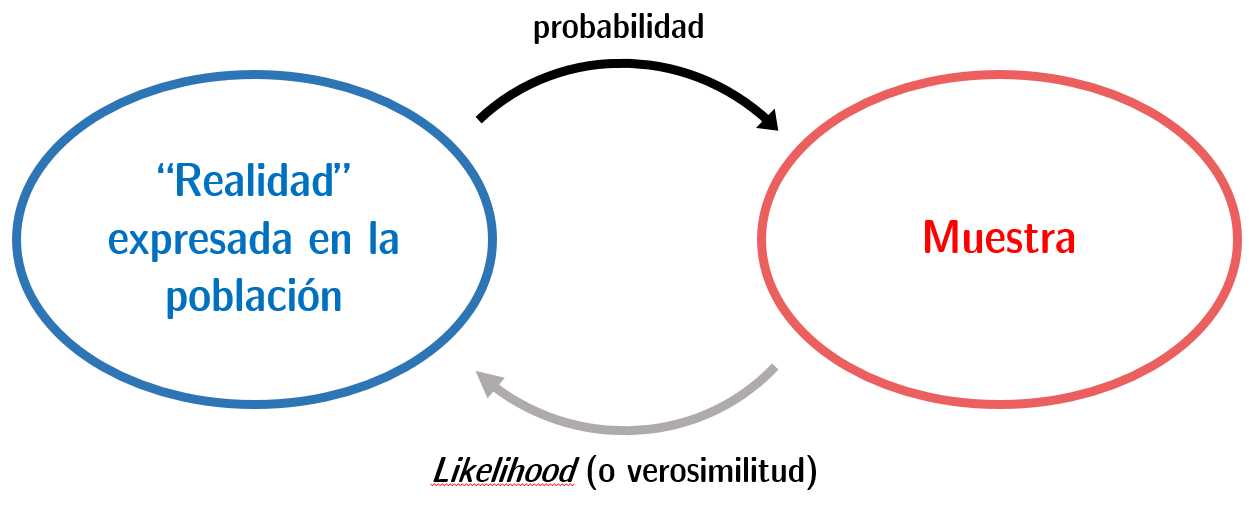
\includegraphics[width=1.2\linewidth]{00-images/fig_7_1}

Cuando tenemos una variable dependiente dicotómica que queremos modelar,
asumimos que la misma tiene una distribución de Bernoulli con una
probabilidad que desconocemos. Así, estimaremos por medio de Máxima
Verosimilitud nuestra probabilidad desconocida dada una combinación
linear determinada de variables independientes (ver figura 2). Un muy
buen ejercicio para comprender como se estima un parámetro cuya
distribución es binomial por medio de Máxima Verosimilitud es ofrecida
por {[}RPubs{]} (\url{https://rpubs.com/felixmay/MLE}).

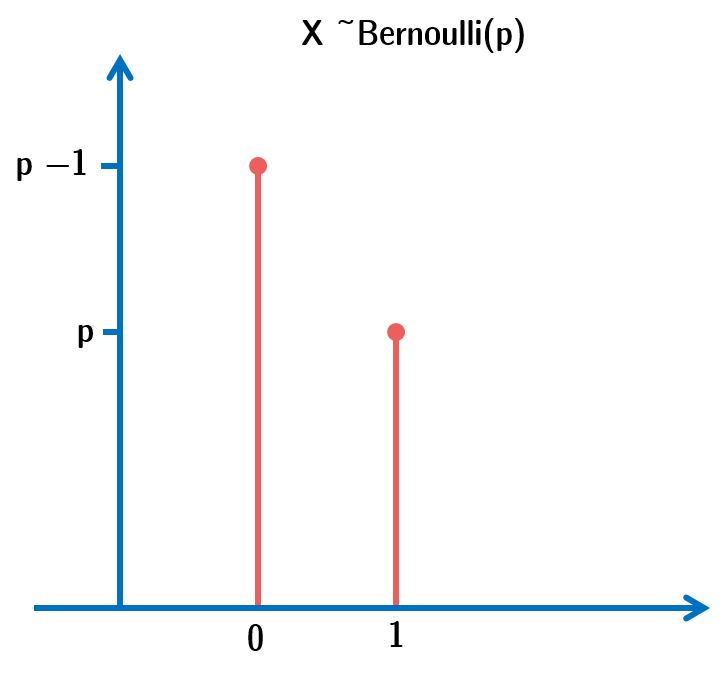
\includegraphics[width=1.2\linewidth]{00-images/fig_7_2}

La Ciencia Política ha hecho extensivo el uso de modelos Logit, por
sobre los modelos Probit, en buena medida debido a que los primeros
permiten el cálculo de razones de oportunidades (\emph{odds ratios}).
Casi todos los manuales econométricos discuten las diferencias y
similitudes entre ambos, las cuales son muchas a los fines prácticos de
estimar un modelo. Por ello, siendo que son métodos que derivan en
resultados muy similares, sólo utilizaremos Logit en este capítulo.
Ambos métodos utilizan funciones de enlace (\emph{link functions})
diferentes y Logit lleva ese nombre debido a que su función está dada
por el logaritmo natural de las razones de oportunidad.

\(ln(odds) = ln(\frac {p}{1 - p})\)

Despejando los términos podemos calcular, de tal forma que obtenemos

\$logit\^{}\{-1\}(\alpha) = \frac {1}{1+e^{-\alpha}} =
\frac {e^\alpha}{1+e^\alpha} \$

Donde es la combinación linear de las variables independientes y sus
coeficientes. La inversa del Logit nos dará la probabilidad de Y ser
igual a 1 dada una cierta combinación de variables independientes. Asi,

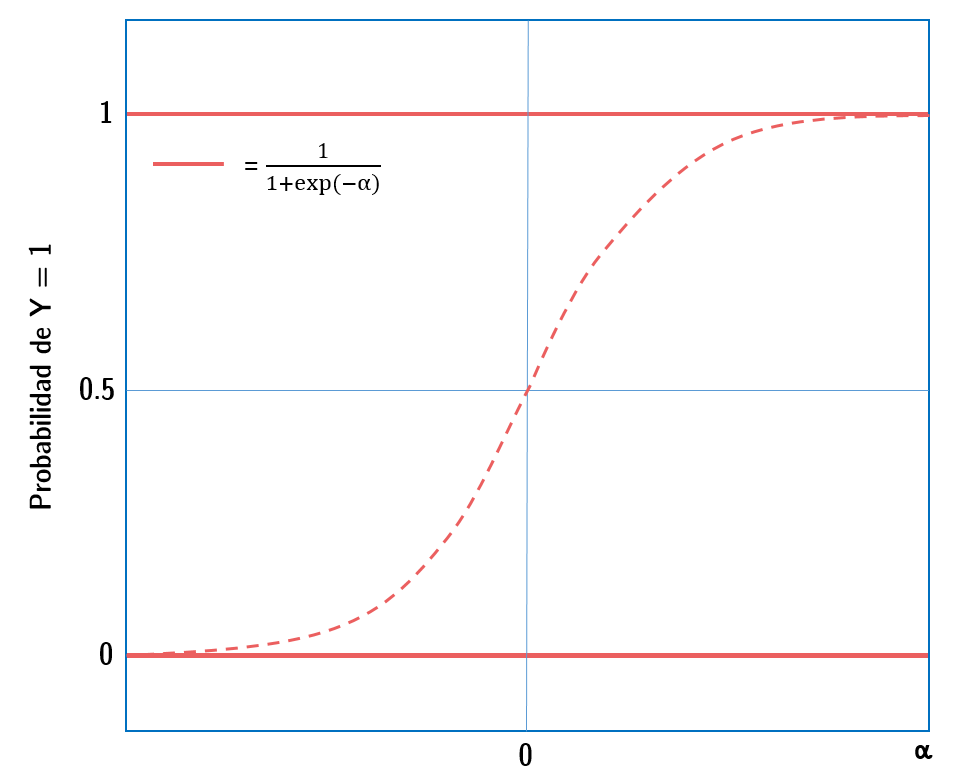
\includegraphics[width=1.2\linewidth]{00-images/fig_7_3}

Nótese que la función es indefinida en 0 y en 1, es decir, la
probabilidad se aproxima infinitamente al límite sin nunca tocarlo.

Los modelos probabilísticos han ganado enorme preeminencia en la Ciencia
Política en los últimos años y es probable que estés buscando una guía
para saber qué hacer y qué no hacer cuando tiene una variable
dependiente dicotómica. Para ello vamos a ilustrar un paso a paso en R
utilizando como ejemplo la base de datos del libro {[}``Democracies and
Dictatorships in Latin America: Emergence, Survival, and Fall'' de Scott
Mainwaring y Aníbal Perez-Liñan (2013){]}
(\url{https://kellogg.nd.edu/democracies-and-dictatorships-latin-america-emergence-survival-and-fall}).
A lo largo del libro los autores analizan qué variables permiten
explicar que a lo largo del siglo XX y comienzos del XXI hayan ocurrido
quiebres democráticos en América Latina. En el capítulo 4 se preguntan
qué factores explican la supervivencia de los regímenes políticos. Si
bien testan varios modelos, algunos logísticos y otros de supervivencia
(que están desarrollados en el Capítulo 10), a los fines prácticos
haremos un ejemplo muy sencillo. Suponiendo que la variable dependiente
asume el valor ``1'' si el país sufre un quiebre de su régimen político
democrático y ``0'' si no, ¿qué efecto tiene sobre la probabilidad de un
quiebre de este tipo ocurrir que un país latinoamericano de mayores
poderes constitucionales al poder ejecutivo? Como argumentan los
autores, se puede medir estos poderes por medio del índice creado por
{[}Shugart y Carey{]}
(\url{http://www.cambridge.org/gb/academic/subjects/politics-international-relations/comparative-politics/presidents-and-assemblies-constitutional-design-and-electoral-dynamics?format=PB\&isbn=9780521429900})
de poder presidencial (1992) que los autores incluyen en su base de
datos. Así,

\begin{Shaded}
\begin{Highlighting}[]
\NormalTok{datos_mp <-}\StringTok{ }\KeywordTok{read_stata}\NormalTok{(}\StringTok{"00-datos/Cap 7_base_mainwaring_perez.dta"}\NormalTok{)}
\end{Highlighting}
\end{Shaded}

\begin{Shaded}
\begin{Highlighting}[]
\KeywordTok{summary}\NormalTok{(datos_mp)}
\end{Highlighting}
\end{Shaded}

\begin{verbatim}
##    country              cc_cow         sc_wb                year     
##  Length:2216        Min.   : 40.0   Length:2216        Min.   :1900  
##  Class :character   1st Qu.: 90.0   Class :character   1st Qu.:1927  
##  Mode  :character   Median :100.0   Mode  :character   Median :1955  
##                     Mean   :106.5                      Mean   :1955  
##                     3rd Qu.:145.0                      3rd Qu.:1983  
##                     Max.   :165.0                      Max.   :2010  
##                                                                      
##     admin                 r                e                f        
##  Length:2216        Min.   :0.0000   Min.   :0.0000   Min.   :0.000  
##  Class :character   1st Qu.:0.0000   1st Qu.:0.0000   1st Qu.:2.000  
##  Mode  :character   Median :0.0000   Median :0.0000   Median :2.000  
##                     Mean   :0.6728   Mean   :0.7811   Mean   :1.888  
##                     3rd Qu.:1.0000   3rd Qu.:2.0000   3rd Qu.:2.000  
##                     Max.   :2.0000   Max.   :2.0000   Max.   :2.000  
##                                                       NA's   :1183   
##        cl             p             trans2         breakdown     
##  Min.   :0.00   Min.   :0.000   Min.   :0.0000   Min.   :0.0000  
##  1st Qu.:1.00   1st Qu.:2.000   1st Qu.:0.0000   1st Qu.:0.0000  
##  Median :2.00   Median :2.000   Median :0.0000   Median :0.0000  
##  Mean   :1.53   Mean   :1.822   Mean   :0.0633   Mean   :0.0485  
##  3rd Qu.:2.00   3rd Qu.:2.000   3rd Qu.:0.0000   3rd Qu.:0.0000  
##  Max.   :2.00   Max.   :2.000   Max.   :2.0000   Max.   :1.0000  
##  NA's   :1183   NA's   :1183    NA's   :968      NA's   :1268    
##       a_1              s_1              age             age2     
##  Min.   :0.0000   Min.   :0.0000   Min.   : 1.00   Min.   :   1  
##  1st Qu.:0.0000   1st Qu.:0.0000   1st Qu.: 5.00   1st Qu.:  25  
##  Median :1.0000   Median :0.0000   Median :12.00   Median : 144  
##  Mean   :0.5683   Mean   :0.1976   Mean   :15.37   Mean   : 391  
##  3rd Qu.:1.0000   3rd Qu.:0.0000   3rd Qu.:22.00   3rd Qu.: 484  
##  Max.   :1.0000   Max.   :1.0000   Max.   :61.00   Max.   :3721  
##  NA's   :20       NA's   :20       NA's   :896     NA's   :896   
##       age3            time3         lntime3            fh        
##  Min.   :     1   Min.   : 0.0   Min.   :0.000   Min.   : 0.000  
##  1st Qu.:   125   1st Qu.: 6.0   1st Qu.:1.946   1st Qu.: 5.000  
##  Median :  1728   Median :13.0   Median :2.639   Median : 8.000  
##  Mean   : 12923   Mean   :13.6   Mean   :2.387   Mean   : 7.158  
##  3rd Qu.: 10648   3rd Qu.:20.0   3rd Qu.:2.996   3rd Qu.: 9.000  
##  Max.   :226981   Max.   :32.0   Max.   :3.466   Max.   :12.000  
##  NA's   :896      NA's   :1694   NA's   :1713    NA's   :1436    
##      aclp2          npr_all           npr_gov           npr_opp       
##  Min.   :1.000   Min.   :-1.0000   Min.   :-1.0000   Min.   :-1.0000  
##  1st Qu.:2.000   1st Qu.:-0.2500   1st Qu.:-0.5000   1st Qu.: 0.0000  
##  Median :2.000   Median : 0.1667   Median : 0.0000   Median : 0.2500  
##  Mean   :2.721   Mean   : 0.1675   Mean   : 0.0978   Mean   : 0.2649  
##  3rd Qu.:4.000   3rd Qu.: 0.5000   3rd Qu.: 0.6667   3rd Qu.: 0.7500  
##  Max.   :4.000   Max.   : 1.0000   Max.   : 1.0000   Max.   : 1.0000  
##  NA's   :996     NA's   :876       NA's   :876       NA's   :876      
##     rad_all          rad_gov          rad_opp          npr_all1      
##  Min.   :0.0000   Min.   :0.0000   Min.   :0.0000   Min.   :-1.0000  
##  1st Qu.:0.1250   1st Qu.:0.0000   1st Qu.:0.0000   1st Qu.:-0.2500  
##  Median :0.3333   Median :0.3333   Median :0.2500   Median : 0.1667  
##  Mean   :0.3945   Mean   :0.3970   Mean   :0.3600   Mean   : 0.1618  
##  3rd Qu.:0.6667   3rd Qu.:0.7500   3rd Qu.:0.6667   3rd Qu.: 0.5000  
##  Max.   :1.0000   Max.   :1.0000   Max.   :1.0000   Max.   : 1.0000  
##  NA's   :876      NA's   :876      NA's   :876      NA's   :896      
##      region          d_nonla              us_t            dif08        
##  Min.   :0.0000   Min.   :-2.59483   Min.   :0.0000   Min.   :-4.0630  
##  1st Qu.:0.1842   1st Qu.:-1.49515   1st Qu.:0.1250   1st Qu.:-0.9838  
##  Median :0.2632   Median : 0.14000   Median :0.2500   Median :-0.1264  
##  Mean   :0.3329   Mean   : 0.02808   Mean   :0.4033   Mean   : 0.6851  
##  3rd Qu.:0.4474   3rd Qu.: 1.38000   3rd Qu.:0.7500   3rd Qu.: 2.4828  
##  Max.   :0.8684   Max.   : 3.22222   Max.   :1.0000   Max.   : 5.8831  
##  NA's   :20       NA's   :100        NA's   :60       NA's   :996      
##       pgdp             gdp_1_          gpgdp                g_1           
##  Min.   :0.04224   Min.   :3.743   Min.   :-0.286233   Min.   :-0.286233  
##  1st Qu.:0.74426   1st Qu.:6.612   1st Qu.:-0.001656   1st Qu.:-0.001656  
##  Median :1.31840   Median :7.184   Median : 0.019615   Median : 0.019615  
##  Mean   :1.90181   Mean   :7.166   Mean   : 0.022346   Mean   : 0.022346  
##  3rd Qu.:2.48104   3rd Qu.:7.816   3rd Qu.: 0.047283   3rd Qu.: 0.047283  
##  Max.   :9.89381   Max.   :9.200   Max.   : 0.531078   Max.   : 0.531078  
##  NA's   :22        NA's   :22      NA's   :22          NA's   :22         
##     ghist10                i              ihist10             wfm        
##  Min.   :-0.143831   Min.   :-0.1084   Min.   :-0.0816   Min.   :0.0000  
##  1st Qu.: 0.005731   1st Qu.: 0.0379   1st Qu.: 0.0520   1st Qu.:0.0032  
##  Median : 0.017613   Median : 0.1027   Median : 0.1232   Median :0.0110  
##  Mean   : 0.022876   Mean   : 0.2277   Mean   : 0.2432   Mean   :0.0486  
##  3rd Qu.: 0.035152   3rd Qu.: 0.2147   3rd Qu.: 0.2277   3rd Qu.:0.0709  
##  Max.   : 0.141336   Max.   : 4.7749   Max.   : 3.8725   Max.   :0.4369  
##  NA's   :1           NA's   :1119      NA's   :1087      NA's   :1508    
##      oilmin          indust_            lit_           gini_      
##  Min.   :0.0000   Min.   : 5.384   Min.   : 8.00   Min.   :29.96  
##  1st Qu.:0.0000   1st Qu.:17.000   1st Qu.:49.60   1st Qu.:46.48  
##  Median :0.0000   Median :22.001   Median :71.46   Median :51.85  
##  Mean   :0.1784   Mean   :21.102   Mean   :66.80   Mean   :51.18  
##  3rd Qu.:0.0000   3rd Qu.:26.222   3rd Qu.:86.64   3rd Qu.:56.50  
##  Max.   :1.0000   Max.   :34.500   Max.   :98.60   Max.   :67.83  
##  NA's   :876      NA's   :896      NA's   :630     NA's   :1551   
##       iac             multip          shugart         d_00_44      
##  Min.   :0.0000   Min.   :0.0000   Min.   : 5.00   Min.   :0.0000  
##  1st Qu.:0.0000   1st Qu.:0.0000   1st Qu.:15.00   1st Qu.:0.0000  
##  Median :0.0000   Median :0.0000   Median :16.00   Median :0.0556  
##  Mean   :0.1221   Mean   :0.3502   Mean   :16.33   Mean   :0.1553  
##  3rd Qu.:0.0000   3rd Qu.:1.0000   3rd Qu.:18.00   3rd Qu.:0.2959  
##  Max.   :1.0000   Max.   :1.0000   Max.   :25.00   Max.   :0.5889  
##  NA's   :996      NA's   :1171     NA's   :1054    NA's   :896     
##    npr_45_77         rad_45_77          npr_t             rad_t       
##  Min.   :-0.6162   Min.   :0.1253   Min.   :-1.8644   Min.   :0.0000  
##  1st Qu.:-0.3458   1st Qu.:0.2654   1st Qu.:-0.4498   1st Qu.:0.5418  
##  Median :-0.0129   Median :0.4610   Median : 0.0182   Median :0.8989  
##  Mean   :-0.0332   Mean   :0.4780   Mean   : 0.0589   Mean   :1.0872  
##  3rd Qu.: 0.1793   3rd Qu.:0.6806   3rd Qu.: 0.5336   3rd Qu.:1.5459  
##  Max.   : 0.8995   Max.   :0.9242   Max.   : 3.1174   Max.   :3.1166  
##  NA's   :1556      NA's   :1556     NA's   :1713      NA's   :1713    
##    idsampler    
##  Min.   :10.00  
##  1st Qu.:21.00  
##  Median :22.00  
##  Mean   :33.71  
##  3rd Qu.:51.00  
##  Max.   :52.00  
##  NA's   :20
\end{verbatim}

\begin{Shaded}
\begin{Highlighting}[]
\NormalTok{modelo_}\DecValTok{1}\NormalTok{ <-}\StringTok{ }\KeywordTok{glm}\NormalTok{(breakdown }\OperatorTok{~}\StringTok{ }\NormalTok{shugart, }
                \DataTypeTok{data   =}\NormalTok{ datos_mp,}
                \DataTypeTok{family =} \KeywordTok{binomial}\NormalTok{(}\StringTok{"logit"}\NormalTok{))}
\end{Highlighting}
\end{Shaded}

\begin{Shaded}
\begin{Highlighting}[]
\KeywordTok{summary}\NormalTok{(modelo_}\DecValTok{1}\NormalTok{)}
\end{Highlighting}
\end{Shaded}

\begin{verbatim}
## 
## Call:
## glm(formula = breakdown ~ shugart, family = binomial("logit"), 
##     data = datos_mp)
## 
## Deviance Residuals: 
##     Min       1Q   Median       3Q      Max  
## -0.7268  -0.2953  -0.2689  -0.2227   2.7917  
## 
## Coefficients:
##             Estimate Std. Error z value Pr(>|z|)   
## (Intercept) -0.23929    0.96383  -0.248  0.80392   
## shugart     -0.19142    0.06477  -2.955  0.00312 **
## ---
## Signif. codes:  0 '***' 0.001 '**' 0.01 '*' 0.05 '.' 0.1 ' ' 1
## 
## (Dispersion parameter for binomial family taken to be 1)
## 
##     Null deviance: 217.84  on 643  degrees of freedom
## Residual deviance: 209.56  on 642  degrees of freedom
##   (1572 observations deleted due to missingness)
## AIC: 213.56
## 
## Number of Fisher Scoring iterations: 6
\end{verbatim}

El coeficiente para la variable \emph{shugart} está negativamente
asociado a la probabilidad de ocurrencia de un quiebre de régimen, y es
estadísticamente significativo (p=0.0026). Ahora bien, a diferencia de
los modelos por MCO del capítulo anterior, donde podíamos interpretar
directamente el efecto de la variable independiente sobre la dependiente
a partir de los coeficientes de la regresión, para el caso de
regresiones logísticas esto no es tan sencillo. Si partimos de que la
función de enlace de logit es el logaritmo de las razones de
oportunidades, tenemos que

\(ln(\frac {p}{1 - p}) = \beta_{0} + \beta_{1}x_{1}\)

Despejando \(ln\), tenemos que

\((\frac {p}{1 - p}) = e^{\beta_{0}+\beta_{1}x_{1}}\)

Y despejando los términos tenemos que

\(\hat{p} = \frac {e^{\beta_{0}+\beta_{1}x_{1}}}{1 + e^{\beta_{0}+\beta_{1}x_{1}}}\)

Lo que queremos, entonces, es transformar los coeficientes tal y como
los reporta R en una probabilidad asociada a que la variable dependiente
asuma el valor ``1''. Sabemos que la variable independiente
(\emph{shugart}) es un índice que a mayor valor, mayor concentración de
poder del ejecutivo \emph{vis a vis} el legislativo, por lo tanto el
coeficiente nos dice que a menor concentración de poder del ejecutivo,
mayor la probabilidad de un quiebre de régimen. En la muestra de los
autores, que cubre 20 países latinoamericanos entre 1900 y 2010, el
índice oscila de un mínimo de 5 (Haití, varios años) a un máximo de 25
(Brasil en 1945) ¿Cómo puedo saber en qué magnitud se afecta la
probabilidad de un quiebre democrático si el nivel de concentración de
poder del ejecutivo pasa de un puntaje de 5 (mínimo) a uno de 25
(máximo)?

\begin{Shaded}
\begin{Highlighting}[]
\KeywordTok{attach}\NormalTok{(datos_mp)}
\KeywordTok{qplot}\NormalTok{(shugart, }\DataTypeTok{geom=}\StringTok{"histogram"}\NormalTok{) }
\end{Highlighting}
\end{Shaded}

\begin{verbatim}
## `stat_bin()` using `bins = 30`. Pick better value with `binwidth`.
\end{verbatim}

\begin{verbatim}
## Warning: Removed 1054 rows containing non-finite values (stat_bin).
\end{verbatim}

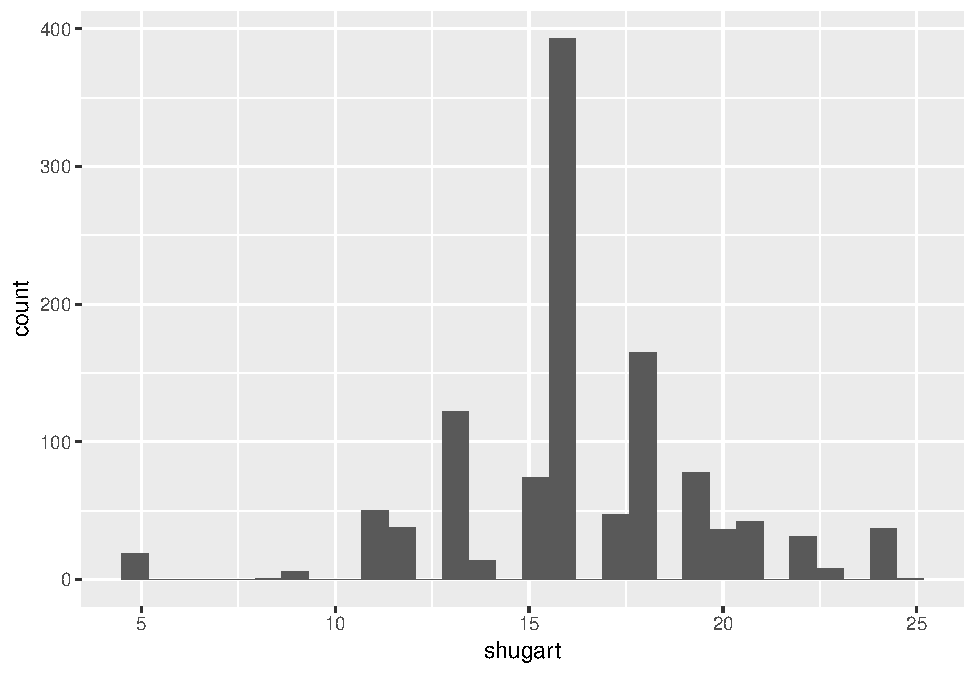
\includegraphics{bookdown-demo_files/figure-latex/unnamed-chunk-58-1.pdf}

Para ello podemos reemplazar los valores de nuestra última fórmula, en
la que hemos aislado en el lado izquierdo de la fórmula a \(\hat {p}\).
Primero debemos calcular cuál es la probabilidad de sufrir un quiebre de
régimen en un nivel de Shugart de 5 y en un nivel 25, respectivamente,
para luego calcular la diferencia. Así tenemos que

\(\hat{p} = \frac {e^{(0+(-0.019*5))}}{1 + e^{(0+(-0.019*5))}}\)

Note que el valor correspondiente al intercepto es igual a 0 pues ese
coeficiente no ha resultado estadísticamente significativo. Sabemos que
para un índice de Shugart y Carey de 5, luego de hacer el cálculo en la
fórmula arriba, la probabilidad es igual a 0.47 o 47\%. Si repetimos el
proceso para un valor de Shugart de 25 la probabilidad cae a 38\%. Con
las probabilidades podemos calcular oportunidades, que son simplemente
\(\frac {p}{1-p}\). De esta manera, la oportunidad (\emph{odd} en
inglés) para un valor 5 del índice de Shugart y Carey es de 0.90
mientras que para un índice de Shugart y Carey de 25 es de 0.62. La
utilidad de las oportunidades es que permite calcular razones de
probabilidades (\emph{odds ratios}). ¿Cuál es la utilidad de una razón
de probabilidades? Si calculo la probabilidad de un cambio en el índice
de Shugart y Carey de 23 a 24 la magnitud será diferente a un cambio en
el índice de 12 a 13, por ejemplo. Es decir, los efectos de la variable
independiente sobre la probabilidad de la variable dependiente ocurrir
no son lineares. Estos dependerán de la curvatura en forma de ``S'' de
la función. Sin embargo, las razones de probabilidades tienen la
propiedad de reflejar cambios independientemente de la curvatura de la
función, es decir, son cambios ``constantes''. Siendo que los modelos
Probit y Logit generan resultados muy similares, pero que apenas los
modelos Logit permiten el cálculo de razones de probabilidad, ésta es la
principal razón por la que la literatura de Ciencia Política se ha
inclinado hacia esta opción. Veamos cómo sería el cálculo de razones de
probabilidad siguiendo el ejemplo que acabamos de crear con la base de
datos de Mainwaring y Perez-Liñan. Dijimos que la oportunidad está dada
por \(\frac {p}{1 - p}\). Una razón de oportunidades se expresaría,
entonces, como \(\frac {\frac {p_1}{1-p_1}}{\frac {p_2}{1-p_2}}\).
Supongamos que Chile en el año 1992 tenía un índice de Shugart de 15, y
que en el año 1993 ese índice subió a 16 (no son valores reales).

\$ Pr(quiebre democrático)\{\emph{\{Chile,1992\}\} =
\frac {e^{(0+(-0.019*15))}}{1 + e^{((0+(-0.019*15))}} = 0.42\$ \$
Pr(quiebre democrático)\{}\{Chile,1993\}\} =
\frac {e^{(0+(-0.019*16))}}{1 + e^{(0+(-0.019*16))}} = 0.43\$

La probabilidad difiere poco y cae en un 2.4\% lo que puede ser un valor
considerable. La razón de oportunidades se calcula como el cociente de
ambas oportunidades, así:

\(\frac {0.42}{0.43}=0.97\)

De esta manera, toda razón de oportunidades mayor a 1 expresa un cambio
positivo, mientras que todo valor menor a 1 (entre 0 y 1) representa un
cambio negativo en las probabilidades estimadas. Si hiciéramos el mismo
ejercicio para otros valores del índice de Shugart y Carey, por ejemplo,
un cambio de 3 a 4 o de 23 a 24, el cociente de las oportunidades daría
0.97. R ofrece paquetes para que este análisis sea fácil de hacerse.
Podemos visualizar fácilmente los cocientes de oportunidades utilizando
el paquete ´sjPlot´, podemos calcular probabilidades predichas, y además
podemos hacer tests para saber la capacidad explicativa de nuestros
modelos. Utilizando la misma base de datos haremos un ejemplo de una
rutina típica, que puedes recrear en casa utilizando tus propios datos.
Los pasos a seguir son (a) estimar los modelos, (b) crear tablas
formateadas para pegar en nuestros procesadores de texto, (c) crear
figuras para visualizar la magnitud de los coeficientes por medio de
cociente de oportunidades, (d) visualizar probabilidades predichas para
variables de interés, (e) calcular capacidad explicativa de los modelos
(porcentaje correctamente predicho, AIC, BIC, curvas ROC, \emph{Brier
scores} o \emph{separation plots}, que explicaremos a continuación).
Cuando uno trabaja con una variable dependiente binaria, y lo que quiere
es rodar algunos modelos logísticos para incorporar a su trabajo,
primero es recomendable utilizar Pacman. \texttt{pacman} es un paquete
de R que hace mucho más fácil trabajar con otros paquetes, pues permite
cargar todos al mismo tiempo. Comencemos por cargarlo:

\begin{Shaded}
\begin{Highlighting}[]
\ControlFlowTok{if}\NormalTok{ (}\OperatorTok{!}\KeywordTok{require}\NormalTok{(}\StringTok{"pacman"}\NormalTok{))}
    \KeywordTok{install.packages}\NormalTok{(}\StringTok{"pacman"}\NormalTok{); }\KeywordTok{library}\NormalTok{(pacman)  }
\end{Highlighting}
\end{Shaded}

\begin{verbatim}
## Loading required package: pacman
\end{verbatim}

\begin{verbatim}
## Warning: package 'pacman' was built under R version 3.4.1
\end{verbatim}

Para que sea simple utilizar la función \texttt{pacman}, recomendamos
añadir \texttt{library(pacman)} a
\href{http://www.statmethods.net/interface/customizing.html}{su archivo
de .Rprofile}, para que se cargue automáticamente cada vez que abra R
Studio. De esta manera no habrá que ejecutarlo cada vez que abra R
Studio. La principal gracia de \texttt{pacman} es su función
\texttt{p\_load}, que nos permite cargar varios paquetes en un solo
comando y, si nos los tenemos instalados, lo hace por nosotros (en el
siguiente paso la utilizaremos). Si no tienes instalados los siguientes
paquetes, \texttt{p\_load} los instalará por ti. Si nos has acompañado
desde los capítulos anteriores, este paso te resultará familiar.

\begin{Shaded}
\begin{Highlighting}[]
\KeywordTok{p_load}\NormalTok{(haven,    }\CommentTok{# parte del tidyverse, para cargar bases de datos en formatos foráneos}
\NormalTok{       verification,}
\NormalTok{       janitor,  }\CommentTok{# nos da la función tabyl(), para hacer tablas tidy}
\NormalTok{       sjPlot,}
\NormalTok{       stargazer, }\CommentTok{# nos ayuda a hacer tablas de modelos de regresión}
\NormalTok{       tidyverse,}
\NormalTok{       pscl,}
\NormalTok{       separationplot}
\NormalTok{       )}
\end{Highlighting}
\end{Shaded}

¿Recuerde el ADP? Una de las funciones que hemos facilitado es la de
creación de tablas editables para artículos académicos utilizando la
función \texttt{stargazer}. Si utilizas nuestro paquete te ahorrarás
muchos pasos que son engorrosos.

\begin{Shaded}
\begin{Highlighting}[]
\KeywordTok{library}\NormalTok{(stargazer)}
\KeywordTok{source}\NormalTok{(}\StringTok{"ADP.R"}\NormalTok{)}
\end{Highlighting}
\end{Shaded}

Por medio de \texttt{stargazer} podemos exportar nuestras tablas
formateadas en html para poder incorporarlas en nuestros artículos
directamente. Para ejemplificar este paso lo que haremos es agregar al
modelo 1 dos modelos más: El modelo 2 tendrá como variables
independientes al índice de Shugart y Carey más la variable \emph{age}
que mide en años la edad del régimen político. qplot(age,
geom=``histogram'')

\begin{Shaded}
\begin{Highlighting}[]
\NormalTok{modelo_}\DecValTok{2}\NormalTok{ <-}\StringTok{ }\KeywordTok{glm}\NormalTok{(breakdown }\OperatorTok{~}\StringTok{ }\NormalTok{shugart}\OperatorTok{+}\NormalTok{age, }
                \DataTypeTok{data   =}\NormalTok{ datos_mp,}
                \DataTypeTok{family =} \KeywordTok{binomial}\NormalTok{(}\StringTok{"logit"}\NormalTok{))}
\end{Highlighting}
\end{Shaded}

\begin{Shaded}
\begin{Highlighting}[]
\KeywordTok{summary}\NormalTok{(modelo_}\DecValTok{2}\NormalTok{)}
\end{Highlighting}
\end{Shaded}

\begin{verbatim}
## 
## Call:
## glm(formula = breakdown ~ shugart + age, family = binomial("logit"), 
##     data = datos_mp)
## 
## Deviance Residuals: 
##     Min       1Q   Median       3Q      Max  
## -0.7336  -0.3020  -0.2656  -0.2178   2.8279  
## 
## Coefficients:
##              Estimate Std. Error z value Pr(>|z|)   
## (Intercept) -0.222202   0.967643  -0.230  0.81838   
## shugart     -0.188970   0.065811  -2.871  0.00409 **
## age         -0.004084   0.019607  -0.208  0.83501   
## ---
## Signif. codes:  0 '***' 0.001 '**' 0.01 '*' 0.05 '.' 0.1 ' ' 1
## 
## (Dispersion parameter for binomial family taken to be 1)
## 
##     Null deviance: 217.84  on 643  degrees of freedom
## Residual deviance: 209.52  on 641  degrees of freedom
##   (1572 observations deleted due to missingness)
## AIC: 215.52
## 
## Number of Fisher Scoring iterations: 6
\end{verbatim}

El modelo 3 agrega a las dos variables del modelo 2 una tercer variable
llamada \emph{fh} que corresponde al
\href{https://freedomhouse.org/report/methodology-freedom-world-2017}{Freedom
House score} de democracia.

\begin{Shaded}
\begin{Highlighting}[]
\KeywordTok{qplot}\NormalTok{(fh, }\DataTypeTok{geom=}\StringTok{"histogram"}\NormalTok{) }
\end{Highlighting}
\end{Shaded}

\begin{verbatim}
## `stat_bin()` using `bins = 30`. Pick better value with `binwidth`.
\end{verbatim}

\begin{verbatim}
## Warning: Removed 1436 rows containing non-finite values (stat_bin).
\end{verbatim}

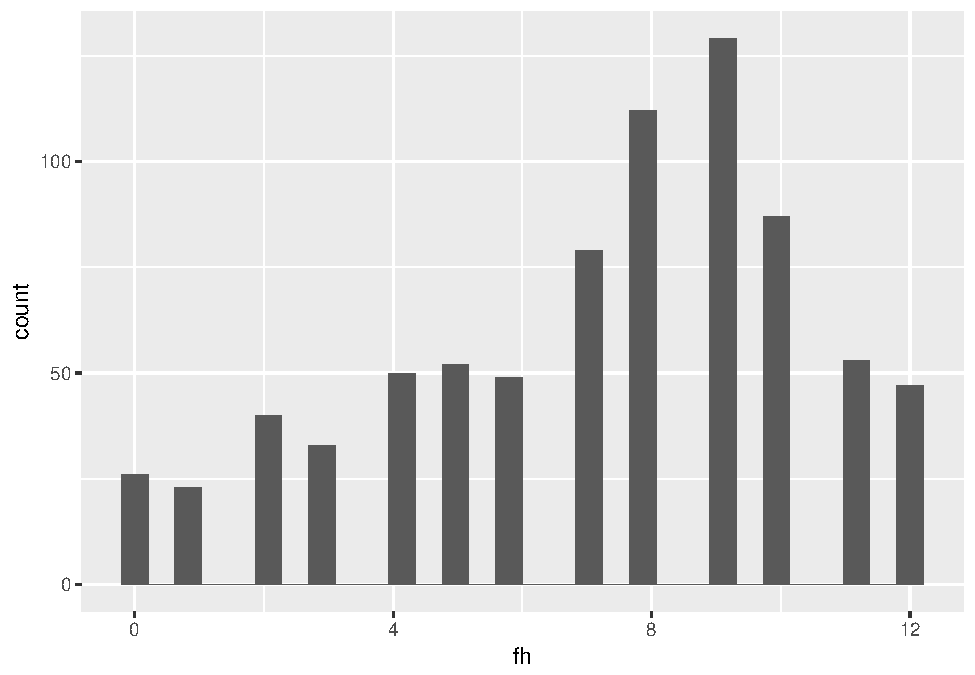
\includegraphics{bookdown-demo_files/figure-latex/unnamed-chunk-64-1.pdf}

\begin{Shaded}
\begin{Highlighting}[]
\NormalTok{modelo_}\DecValTok{3}\NormalTok{ <-}\StringTok{ }\KeywordTok{glm}\NormalTok{(breakdown }\OperatorTok{~}\StringTok{ }\NormalTok{shugart}\OperatorTok{+}\NormalTok{age}\OperatorTok{+}\NormalTok{fh, }
                \DataTypeTok{data   =}\NormalTok{ datos_mp,}
                \DataTypeTok{family =} \KeywordTok{binomial}\NormalTok{(}\StringTok{"logit"}\NormalTok{))}
\end{Highlighting}
\end{Shaded}

\begin{verbatim}
## Warning: glm.fit: fitted probabilities numerically 0 or 1 occurred
\end{verbatim}

\begin{Shaded}
\begin{Highlighting}[]
\KeywordTok{summary}\NormalTok{(modelo_}\DecValTok{3}\NormalTok{)}
\end{Highlighting}
\end{Shaded}

\begin{verbatim}
## 
## Call:
## glm(formula = breakdown ~ shugart + age + fh, family = binomial("logit"), 
##     data = datos_mp)
## 
## Deviance Residuals: 
##      Min        1Q    Median        3Q       Max  
## -1.78635  -0.00080  -0.00007  -0.00001   1.89399  
## 
## Coefficients:
##             Estimate Std. Error z value Pr(>|z|)  
## (Intercept)  15.3596     6.5842   2.333   0.0197 *
## shugart      -0.2173     0.1656  -1.312   0.1894  
## age           0.1664     0.1123   1.482   0.1384  
## fh           -3.7480     1.5051  -2.490   0.0128 *
## ---
## Signif. codes:  0 '***' 0.001 '**' 0.01 '*' 0.05 '.' 0.1 ' ' 1
## 
## (Dispersion parameter for binomial family taken to be 1)
## 
##     Null deviance: 71.271  on 421  degrees of freedom
## Residual deviance: 12.113  on 418  degrees of freedom
##   (1794 observations deleted due to missingness)
## AIC: 20.113
## 
## Number of Fisher Scoring iterations: 12
\end{verbatim}

Una vez creados los tres modelos de interés, los agrupamos en una lista
por medio de la función ´list´.

\begin{Shaded}
\begin{Highlighting}[]
\NormalTok{mp_modelos <-}\StringTok{ }\KeywordTok{list}\NormalTok{(modelo_}\DecValTok{1}\NormalTok{, }
\NormalTok{                   modelo_}\DecValTok{2}\NormalTok{,}
\NormalTok{                   modelo_}\DecValTok{3}\NormalTok{)}
\end{Highlighting}
\end{Shaded}

Para exportar la tabla a html demos definir la opción \textbf{type} y un
nombre para el archivo html en la opción \textbf{out}. Así el comando
sería

stargazer\_easy\_binary(mp\_modelos, type = ``html'', \# OJO out =
``output/tabla\_mp\_modelos.htm'', \# OJO report = ``vct*``, title
=''Modelos 1-3 en base a Mainwaring y Perez Liñan (2013)``, align =
TRUE, dep.var.labels = c(''Quiebre de régimen``), covariate.labels =c
(''Indice de Shugart \& Carey (1992)``,''Edad del régimen``,''Freedom
House``), no.space = TRUE) )

A simple vista observamos que \emph{shugart} deja de ser
estadísticamente significativa cuando controlamos por \emph{fh} y,
además, ésta pasa a ser la única variable estadísticamente significativa
en el tercer modelo. Vemos como el número de observaciones cae
significativamente al incluir la variable \emph{fh} lo que hace difícil
comparar los modelos. Entonces al obtener una tabla como la que acabamos
de crear tenemos dos desafíos: comparar los modelos para saber cuál
tiene mejor ajuste, y saber si la magnitud de los efectos es substantiva
desde un punto de vista científico (por ejemplo, si la variable
\emph{fh} resulta estadísticamente significativa pero la probabilidad de
un quiebre de régimen cae en 0.03\% si un país pasa del peor score de
\emph{fh} al mejor, entonces diríamos que, a pesar de estadísticamente
significativa, nuestra variable carece de significancia substantiva).
Jane Miller hace mucho énfasis en su {[}libro{]}
(\url{http://www.press.uchicago.edu/ucp/books/book/chicago/C/bo15506942.html})
respecto a la diferencia entre significancia estadística y significancia
substantiva: no por ser una variable significativa estadísticamente la
magnitud del efecto será el esperado. Para explorar las magnitudes de
los coeficientes vamos a concentrarnos en el tercer modelo. Una tabla
individual, podrán anticipar, se haría así:

stargazer\_easy\_binary(modelo\_3, type = ``text'', report = ``vct*``,
title =''Modelo 3 en base Mainwaring y Perez Liñan (2013)``, )

Comencemos reemplazando los coeficientes en la tabla por cocientes de
oportunidades. Noten cómo el procedimiento es muy similar al de
reemplazar errores estándar:

stargazer\_easy\_binary(modelo\_3, type = ``text'', report = ``vct*``,
title =''Modelo 3 en base Mainwaring y Perez Liñan (2013), odds
ratios``, coef = list(exp(modelo\_3\$coefficients)))

Podemos representar visualmente lo anterior con la función
\texttt{sjp.glm()} del paquete \texttt{sjPlot}:

\begin{Shaded}
\begin{Highlighting}[]
\KeywordTok{sjp.glm}\NormalTok{(modelo_}\DecValTok{3}\NormalTok{, }
        \DataTypeTok{show.ci     =}\NormalTok{ T,}
        \DataTypeTok{title       =} \StringTok{"Modelo 3 en base Mainwaring y Perez Liñan (2013), odds ratios"}\NormalTok{)}
\end{Highlighting}
\end{Shaded}

\begin{verbatim}
## Warning: glm.fit: fitted probabilities numerically 0 or 1 occurred

## Warning: glm.fit: fitted probabilities numerically 0 or 1 occurred

## Warning: glm.fit: fitted probabilities numerically 0 or 1 occurred

## Warning: glm.fit: fitted probabilities numerically 0 or 1 occurred

## Warning: glm.fit: fitted probabilities numerically 0 or 1 occurred

## Warning: glm.fit: fitted probabilities numerically 0 or 1 occurred

## Warning: glm.fit: fitted probabilities numerically 0 or 1 occurred

## Warning: glm.fit: fitted probabilities numerically 0 or 1 occurred

## Warning: glm.fit: fitted probabilities numerically 0 or 1 occurred

## Warning: glm.fit: fitted probabilities numerically 0 or 1 occurred

## Warning: glm.fit: fitted probabilities numerically 0 or 1 occurred

## Warning: glm.fit: fitted probabilities numerically 0 or 1 occurred

## Warning: glm.fit: fitted probabilities numerically 0 or 1 occurred

## Warning: glm.fit: fitted probabilities numerically 0 or 1 occurred

## Warning: glm.fit: fitted probabilities numerically 0 or 1 occurred

## Warning: glm.fit: fitted probabilities numerically 0 or 1 occurred

## Warning: glm.fit: fitted probabilities numerically 0 or 1 occurred

## Warning: glm.fit: fitted probabilities numerically 0 or 1 occurred

## Warning: glm.fit: fitted probabilities numerically 0 or 1 occurred

## Warning: glm.fit: fitted probabilities numerically 0 or 1 occurred

## Warning: glm.fit: fitted probabilities numerically 0 or 1 occurred

## Warning: glm.fit: fitted probabilities numerically 0 or 1 occurred

## Warning: glm.fit: fitted probabilities numerically 0 or 1 occurred

## Warning: glm.fit: fitted probabilities numerically 0 or 1 occurred

## Warning: glm.fit: fitted probabilities numerically 0 or 1 occurred

## Warning: glm.fit: fitted probabilities numerically 0 or 1 occurred

## Warning: glm.fit: fitted probabilities numerically 0 or 1 occurred

## Warning: glm.fit: fitted probabilities numerically 0 or 1 occurred

## Warning: glm.fit: fitted probabilities numerically 0 or 1 occurred

## Warning: glm.fit: fitted probabilities numerically 0 or 1 occurred

## Warning: glm.fit: fitted probabilities numerically 0 or 1 occurred

## Warning: glm.fit: fitted probabilities numerically 0 or 1 occurred

## Warning: glm.fit: fitted probabilities numerically 0 or 1 occurred
\end{verbatim}

\begin{verbatim}
## Warning in sjp.glm(modelo_3, show.ci = T, title = "Modelo 3 en base
## Mainwaring y Perez Liñan (2013), odds ratios"): Exp. coefficients and/or
## exp. confidence intervals may be out of printable bounds. Consider using
## `axis.lim` argument!
\end{verbatim}

\begin{verbatim}
## Warning: Removed 1 rows containing missing values (geom_errorbar).
\end{verbatim}

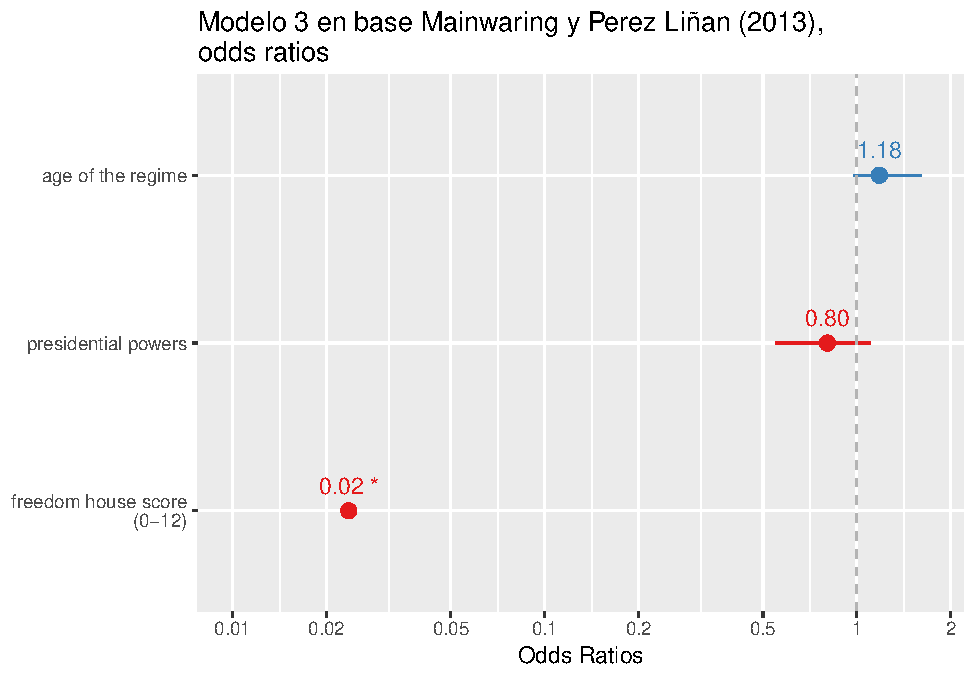
\includegraphics{bookdown-demo_files/figure-latex/unnamed-chunk-68-1.pdf}
Esta figura es mucho más intuitiva de leerse que los coeficientes de las
tablas. En muchas ocasiones es preferible utilizar este tipo de figuras
a tablas. La {[}tendencia{]}
(\url{https://www.princeton.edu/~jkastell/Tables2Graphs/graphs.pdf}) en
la disciplina es a la de prescindir de tablas cuando estas no sean
esenciales. La ciencia política no prestó demasiada atención a la
presentación de resultados por medio de figuras hasta hace unas dos
décadas, y hoy en día con software como R es muy simple de hacer. Un
precursor en la disciplina fue {[}Edward Tufte{]}
(\url{http://pages.mtu.edu/~hcking/Tufte_hKing.pdf}). Con el argumento
\texttt{type\ =\ "slope"} en \texttt{sjp.glm()} podemos apreciar cómo es
la relación entre cada variable independiente y la variable dependiente,
cuando las demás variables independientes están en 0.

\begin{Shaded}
\begin{Highlighting}[]
\KeywordTok{sjp.glm}\NormalTok{(modelo_}\DecValTok{3}\NormalTok{,}
        \DataTypeTok{type        =} \StringTok{"slope"}\NormalTok{,}
        \DataTypeTok{show.ci     =} \OtherTok{TRUE}\NormalTok{,}
        \DataTypeTok{title       =} \StringTok{"Modelo 3 en base Mainwaring y Perez Liñan (2013), pr. predichas con otras variables en 0"}\NormalTok{)}
\end{Highlighting}
\end{Shaded}

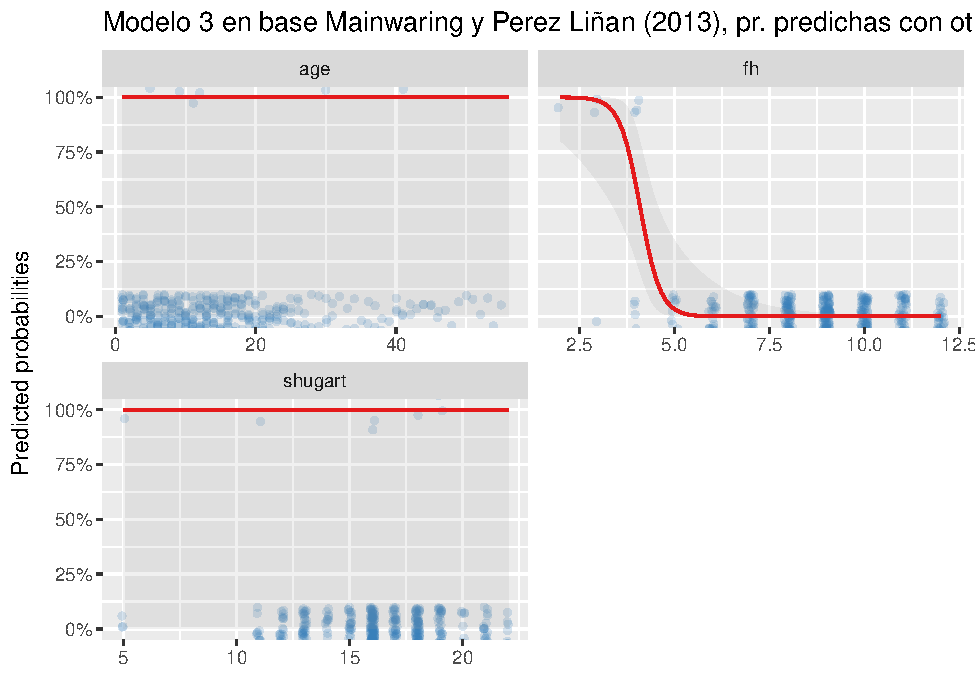
\includegraphics{bookdown-demo_files/figure-latex/unnamed-chunk-69-1.pdf}
Con el argumento \texttt{type\ =\ "pred"} en \texttt{sjp.glm()} podemos
apreciar cómo es la relación entre cada variable independiente y la
variable dependiente, cuando las demás variables independientes están en
sus medias

\begin{Shaded}
\begin{Highlighting}[]
\KeywordTok{sjp.glm}\NormalTok{(modelo_}\DecValTok{3}\NormalTok{, }
        \DataTypeTok{type        =} \StringTok{"pred"}\NormalTok{,}
        \DataTypeTok{show.ci     =} \OtherTok{TRUE}\NormalTok{,}
        \DataTypeTok{vars        =} \StringTok{"fh"}\NormalTok{,}
        \DataTypeTok{title       =} \StringTok{"Modelo 3 en base Mainwaring y Perez Liñan (2013), pr. predichas con otras variables en sus medias"}\NormalTok{)}
\end{Highlighting}
\end{Shaded}

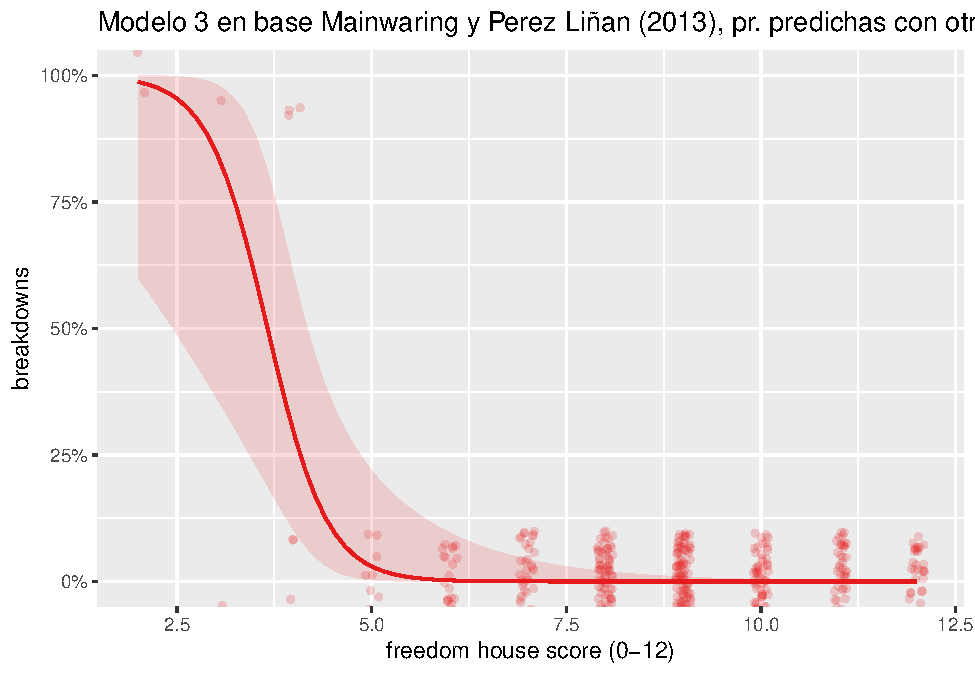
\includegraphics{bookdown-demo_files/figure-latex/unnamed-chunk-70-1.pdf}
Con el argumento \texttt{type\ =\ "eff"} en \texttt{sjp.glm()} podemos
calcular efectos marginales de cada variable independiente en relación a
la variable dependiente, dejando las demás variables independientes
están en sus medias. El efecto marginal es el incremento previsto de la
variable dependiente asociada al aumento de una unidad en una de las
variables independientes, manteniendo las otras constantes. En la
regresión lineal, es solo el parámetro beta. En la regresión logística,
depende del valor de la variable independiente.

\begin{Shaded}
\begin{Highlighting}[]
\KeywordTok{sjp.glm}\NormalTok{(modelo_}\DecValTok{3}\NormalTok{, }
        \DataTypeTok{type        =} \StringTok{"eff"}\NormalTok{,}
        \DataTypeTok{show.ci     =} \OtherTok{TRUE}\NormalTok{,}
        \DataTypeTok{title       =} \StringTok{"Modelo 3 en base Mainwaring y Perez Liñan (2013), efectos marginales"}\NormalTok{)}
\end{Highlighting}
\end{Shaded}

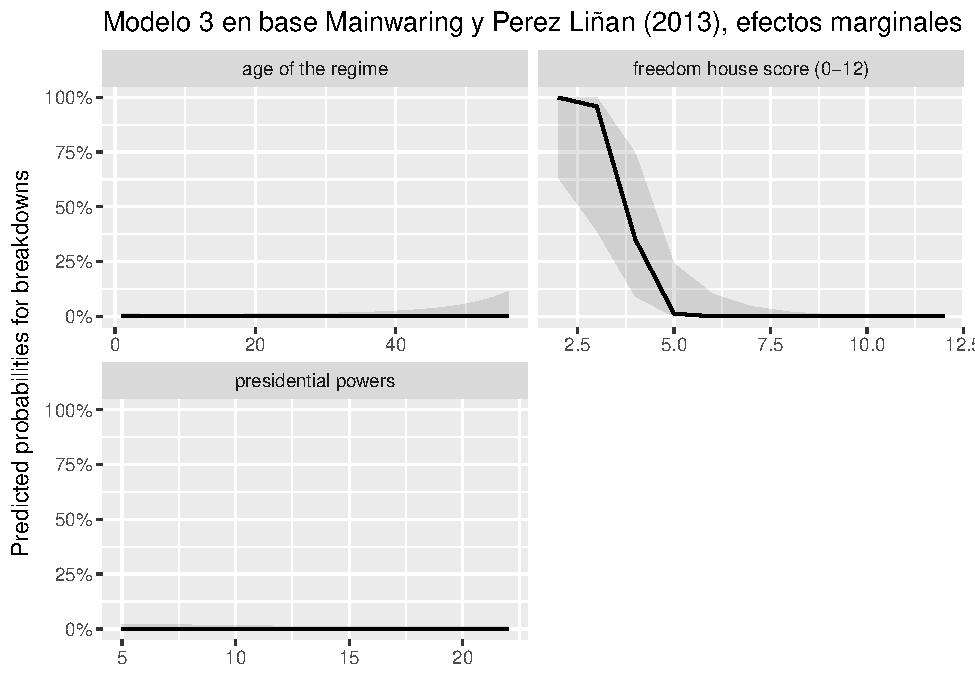
\includegraphics{bookdown-demo_files/figure-latex/unnamed-chunk-71-1.pdf}
Una vez que uno ha analizado la significancia substantiva de los modelos
por medio de figuras analizando las probabilidades predichas y los
efectos marginales, podemos explorar el ajuste de los modelos. Así como
en MCO podemos usar el \(R^2\) y el \emph{Mean Root Square Error}
,existe una serie de estadísticas diseñadas para saber cuál de los
modelos logísticos tiene mejor fit.

stargazer\_easy\_binary(mp\_modelos, type = ``text'', report = ``vct*``,
title =''Modelos 1-3 en base Mainwaring y Perez Liñan (2013)" )

El \emph{wrapper} que hemos creado ya nos provee de varios indicadores
de ajuste, que también podemos calcular por separado:

\subsection{\texorpdfstring{\(Pseudo-R^2\)}{Pseudo-R\^{}2}}\label{pseudo-r2}

Para entender como e interpreta el Pseudo-\(R^2\) (normalmente se usa el
de McFadden) es importante compreender como se diferencia de um \(R^2\)
por MCO (usar este link para R2 em el cap de OLS
\url{http://setosa.io/ev/ordinary-least-squares-regression/}). La
fórmula, en este caso es
\(Pseudo-R^2= 1-\frac {ln \hat{L}(Modelo completo)}{ln \hat{L}(Modelo sólo con intercepto)}\)
Donde \(\hat{L}\) es la verosimilitud estimada por el modelo.
Básicamente, lo que la fórmula está haciendo es comparar el modelo con
todas nuestras covariables al modelo que apenas tiene el intercepto,
para ver cuanto mejora la capacidad explicativa del mismo. Como \(L\)
está entre 0 y 1, su log es menor o igual a 0. Así, cuanto menor la
razón, mayor la diferencia entre el modelo elegido y el modelo con
apenas el intercepto.

\begin{Shaded}
\begin{Highlighting}[]
\KeywordTok{pR2}\NormalTok{(modelo_}\DecValTok{1}\NormalTok{)[[}\StringTok{"McFadden"}\NormalTok{]]}
\end{Highlighting}
\end{Shaded}

\begin{verbatim}
## [1] 0.4306823
\end{verbatim}

\begin{Shaded}
\begin{Highlighting}[]
\KeywordTok{pR2}\NormalTok{(modelo_}\DecValTok{2}\NormalTok{)[[}\StringTok{"McFadden"}\NormalTok{]]}
\end{Highlighting}
\end{Shaded}

\begin{verbatim}
## [1] 0.4308023
\end{verbatim}

\begin{Shaded}
\begin{Highlighting}[]
\KeywordTok{pR2}\NormalTok{(modelo_}\DecValTok{3}\NormalTok{)[[}\StringTok{"McFadden"}\NormalTok{]]}
\end{Highlighting}
\end{Shaded}

\begin{verbatim}
## [1] 0.9670939
\end{verbatim}

También se podría implementar un \(Pseudo-R^2\) ajustado, es decir, una
versión que penalice por cantidad de covaraibles. Siendo que \(c\) es
cantidad de covariables, tenemos que
\(Pseudo-R^2= 1-\frac {ln \hat{L}(Modelo completo)-c}{ln \hat{L}(Modelo sólo con intercepto)}\)

\subsection{AIC}\label{aic}

El Akaike Information Criterion (AIC) también usa información de
\(ln(\hat {L})\) como el \(Pseudo-R^2\). El AIC lo que hace es medir la
``distancia'' que existe entre los verdaderos parámetros y los
estimadores del modelo, por medio de la distancia de Kullback-Leibler.
Por ello, cuanto menor esta distancia, mejor el modelo. Es muy útil a la
hora de comparar diferentes modelos. Se calcula como
\(AIC = 2p-2ln(\hat {L})\) Donde \(p\) es la cantidad de regresores
incluyendo al intercepto, y \(\hat{L}\) es la verosimilitud estimada por
el modelo.

\begin{Shaded}
\begin{Highlighting}[]
\KeywordTok{AIC}\NormalTok{(modelo_}\DecValTok{1}\NormalTok{)}
\end{Highlighting}
\end{Shaded}

\begin{verbatim}
## [1] 213.5639
\end{verbatim}

\begin{Shaded}
\begin{Highlighting}[]
\KeywordTok{AIC}\NormalTok{(modelo_}\DecValTok{2}\NormalTok{)}
\end{Highlighting}
\end{Shaded}

\begin{verbatim}
## [1] 215.5197
\end{verbatim}

\begin{Shaded}
\begin{Highlighting}[]
\KeywordTok{AIC}\NormalTok{(modelo_}\DecValTok{3}\NormalTok{)}
\end{Highlighting}
\end{Shaded}

\begin{verbatim}
## [1] 20.11261
\end{verbatim}

\subsection{BIC}\label{bic}

BIC (Bayesian information criterion) al igual que AIC es un criterio de
comparación de modelos según su ajuste. A los fines prácticos, y para no
entrar en las diferencias entre AIC y BIC, es importante saber que BIC
penaliza de manera más rigurosa que AIC la complejidad del modelo,
siendo que su fórmula es \(BIC=ln(n)p-2ln(\hat {L})\) donde agrega a la
formula \(n\) que es el número de observaciones en la muestra.

\begin{Shaded}
\begin{Highlighting}[]
\KeywordTok{BIC}\NormalTok{(modelo_}\DecValTok{1}\NormalTok{)}
\end{Highlighting}
\end{Shaded}

\begin{verbatim}
## [1] 222.4993
\end{verbatim}

\begin{Shaded}
\begin{Highlighting}[]
\KeywordTok{BIC}\NormalTok{(modelo_}\DecValTok{2}\NormalTok{)}
\end{Highlighting}
\end{Shaded}

\begin{verbatim}
## [1] 228.9228
\end{verbatim}

\begin{Shaded}
\begin{Highlighting}[]
\KeywordTok{BIC}\NormalTok{(modelo_}\DecValTok{3}\NormalTok{)}
\end{Highlighting}
\end{Shaded}

\begin{verbatim}
## [1] 36.29263
\end{verbatim}

\subsection{Brier Score}\label{brier-score}

Ésta es otra medida de ajuste. Cuanto más próximo el score de Brier a 0,
mejor el ajuste del modelo. En general uno no utiliza todas (AIC, BIC,
Brier, etc) sino que elige dos o tres que sean de su agrado. El Brier se
utiliza poco en ciencia política, pero es bastante común en
epidemiología. Creemos que situaciones en que se quiere ``castigar''
mucho las predicciones erróneas, ésta es una alternativa ideal ya que su
fórmula viene dada por \(B=frac\{1}{N} \sum(\hat{p} - x)^2\) Donde \(N\)
es el número de observaciones, \(\hat{p}\) es la probabilidad predicha
para cada observación, y \(x\) es el valor real de la observación en
nuestra base de datos. El score es el promedio para todas las
observaciones de la muestra. ¿Cuál de los tres modelos tiene menor
score?

brier\_score(modelo\_1) brier\_score(modelo\_2) brier\_score(modelo\_3)

\subsection{Porcentaje de predicciones
correctas}\label{porcentaje-de-predicciones-correctas}

Para entender el porcentaje de predicciones correctas en un modelo es
importante tener en claro que un modelo produce cuatro combinaciones
posibles:

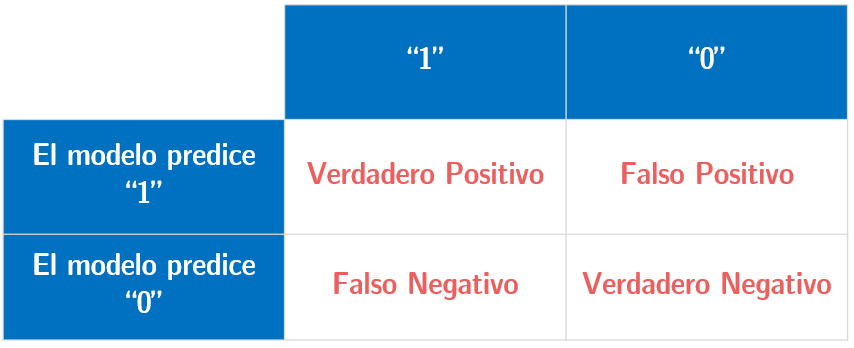
\includegraphics[width=1.2\linewidth]{00-images/fig_7_4} Toda
observación será clasificada como ``correcta'' si corresponde a la
casilla superior izquierda (verdadero positivo) o a la inferior derecha
(verdadero negativo). El porcentaje de observaciones que pertenecen a
estas dos casillas determina el porcentaje de predicciones correctas en
el modelo. Como criterio estándar, si la probabilidad estimada para una
observación es mayor o igual a 50\% se estima que es una probabilidad
positiva, y si es menor a 50\% será una probabilidad negativa.

corr\_pred\_binary(modelo\_1, type = ``prop'')
corr\_pred\_binary(modelo\_2, type = ``prop'')
corr\_pred\_binary(modelo\_3, type = ``prop'')

\subsection{ROC plot}\label{roc-plot}

Las curvas de ROC tienen la ventaja de no definir un límite arbitrario a
partir del cual se decide si la observación ha sido correcta o
incorrectamente clasificada. Su desventaja es que es una figura extra
que deberemos incluir en nuestro artículo (¿quizás pensemos en un
apéndice?). Para interpretar estas figuras, lo que nos interesa es el
área debajo de la curva. A mayor el área bajo la curva, mejor el ajuste
del modelo. Si quieren leer más al respecto, el área conforma un score
que se denomina AUC score (que viene de ``Area Under the Curve''). Vamos
a construirlo con la función \texttt{roc.plot()} del paquete
\texttt{verification}

\begin{Shaded}
\begin{Highlighting}[]
\KeywordTok{roc.plot}\NormalTok{(}\DataTypeTok{x    =}\NormalTok{ modelo_}\DecValTok{1}\OperatorTok{$}\NormalTok{y, }\CommentTok{# tienen el mismo x!}
         \DataTypeTok{pred =} \KeywordTok{cbind}\NormalTok{(}\KeywordTok{predict.glm}\NormalTok{(modelo_}\DecValTok{1}\NormalTok{, }\DataTypeTok{type=}\StringTok{"response"}\NormalTok{),}
                      \KeywordTok{predict.glm}\NormalTok{(modelo_}\DecValTok{2}\NormalTok{, }\DataTypeTok{type=}\StringTok{"response"}\NormalTok{),}
                      \KeywordTok{predict.glm}\NormalTok{(modelo_}\DecValTok{3}\NormalTok{, }\DataTypeTok{type=}\StringTok{"response"}\NormalTok{)),}
         \DataTypeTok{threshold =} \KeywordTok{seq}\NormalTok{(}\DecValTok{0}\NormalTok{,}\DecValTok{1}\NormalTok{, }\FloatTok{0.1}\NormalTok{),}\DataTypeTok{legend =}\NormalTok{ T, }\DataTypeTok{show.thres =}\NormalTok{ F,}
         \DataTypeTok{xlab=}\StringTok{"Ratio de falsas alarmas"}\NormalTok{, }
         \DataTypeTok{ylab=}\StringTok{"Ratio de aciertos"}\NormalTok{,}
         \DataTypeTok{leg.text =} \KeywordTok{c}\NormalTok{(}\StringTok{"Modelo 1"}\NormalTok{,}\StringTok{"Modelo 2"}\NormalTok{, }\StringTok{"Modelo 3"}\NormalTok{), }
         \DataTypeTok{main=}\StringTok{"ROC plot - Modelos 1-3 en base a Mainwaring y Perez Liñan (2013)"}\NormalTok{)}
\end{Highlighting}
\end{Shaded}

\begin{verbatim}
## Warning in cbind(predict.glm(modelo_1, type = "response"),
## predict.glm(modelo_2, : number of rows of result is not a multiple of
## vector length (arg 3)
\end{verbatim}

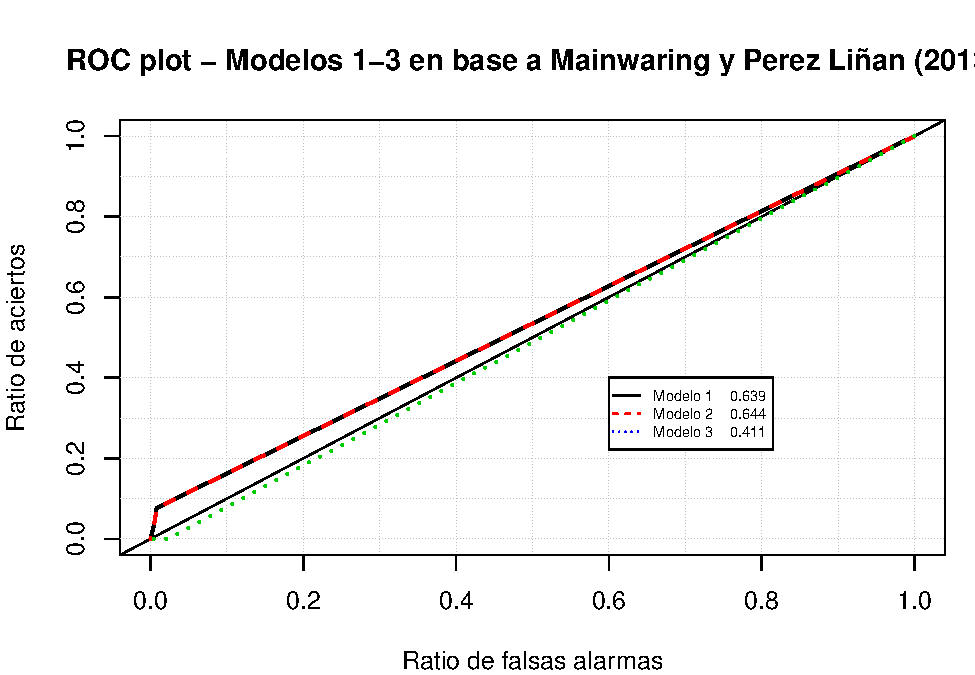
\includegraphics{bookdown-demo_files/figure-latex/unnamed-chunk-76-1.pdf}

En el eje vertical tenemos la \emph{sensibilidad} del modelo mientras
que en el eje horizontal tenemos (1-\emph{especificidad}) del modelo. La
sensibilidad es la razón entre los verdaderos positivos (o sea, aquellas
observaciones predichas como ``1'', que realmente eran ``1'' en la base
de datos), y la suma de los verdaderos postivos más los falsos negativos
(aquellos preichos como ``0'' que en verdad eran ``1''). La
especificidad es la razón entre los verdaderos negativos (aquellas
observaciones predichas como ``0'' que eran ``0'' en la base de datos) y
la suma de los falsos positivos (aquellas observaciones predichas como
``1'' que en verdad eran ``0'') sumado a los verdaderos negativos.

\subsection{Separation plots}\label{separation-plots}

Nótese cómo ocupamos el argumento \texttt{type\ =\ "bands"}, en tanto
nuestro n es muy alto.

\begin{Shaded}
\begin{Highlighting}[]
\KeywordTok{separationplot}\NormalTok{(}\DataTypeTok{pred    =} \KeywordTok{predict.glm}\NormalTok{(modelo_}\DecValTok{1}\NormalTok{, }\DataTypeTok{type =} \StringTok{"response"}\NormalTok{),}
               \DataTypeTok{actual  =} \KeywordTok{as.vector}\NormalTok{(modelo_}\DecValTok{1}\OperatorTok{$}\NormalTok{y),}
               \DataTypeTok{type    =} \StringTok{"bands"}\NormalTok{,}
               \DataTypeTok{newplot =}\NormalTok{ F, }
               \DataTypeTok{heading =} \StringTok{"Separation plot - Modelo 1 en base a Mainwaring y Perez Liñan (2013)"}\NormalTok{)}
\end{Highlighting}
\end{Shaded}

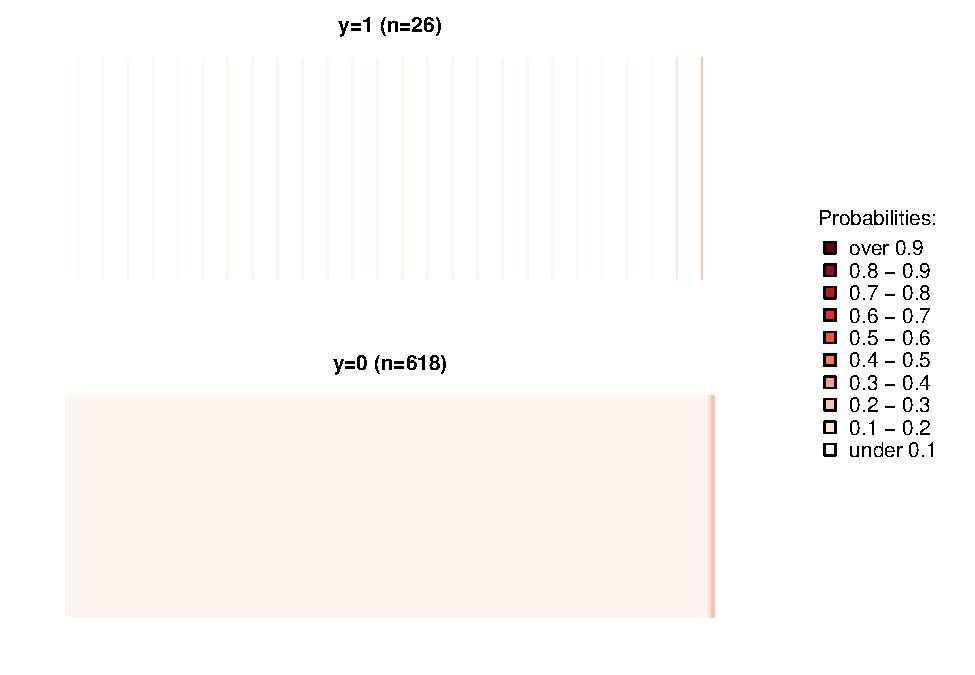
\includegraphics{bookdown-demo_files/figure-latex/unnamed-chunk-77-1.pdf}

\begin{Shaded}
\begin{Highlighting}[]
\KeywordTok{separationplot}\NormalTok{(}\DataTypeTok{pred    =} \KeywordTok{predict.glm}\NormalTok{(modelo_}\DecValTok{2}\NormalTok{, }\DataTypeTok{type =} \StringTok{"response"}\NormalTok{),}
               \DataTypeTok{actual  =} \KeywordTok{as.vector}\NormalTok{(modelo_}\DecValTok{2}\OperatorTok{$}\NormalTok{y),}
               \DataTypeTok{type    =} \StringTok{"bands"}\NormalTok{,}
               \DataTypeTok{newplot =}\NormalTok{ F, }
               \DataTypeTok{heading =} \StringTok{"Separation plot - Modelo 2 en base a a Mainwaring y Perez Liñan (2013)"}\NormalTok{)}
\end{Highlighting}
\end{Shaded}

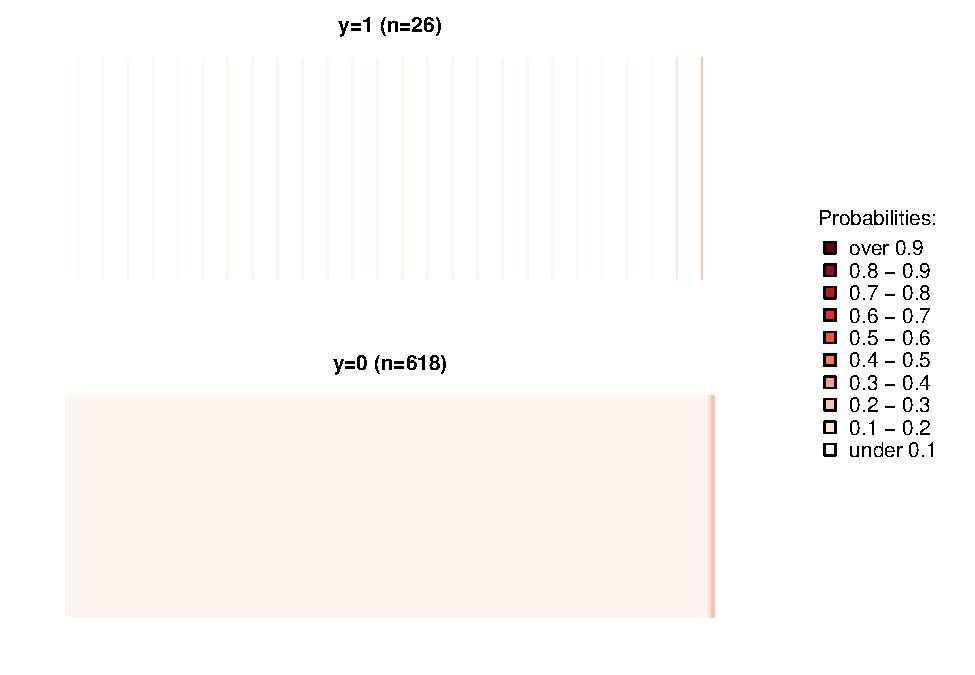
\includegraphics{bookdown-demo_files/figure-latex/unnamed-chunk-78-1.pdf}

\begin{Shaded}
\begin{Highlighting}[]
\KeywordTok{separationplot}\NormalTok{(}\DataTypeTok{pred    =} \KeywordTok{predict.glm}\NormalTok{(modelo_}\DecValTok{3}\NormalTok{, }\DataTypeTok{type =} \StringTok{"response"}\NormalTok{),}
               \DataTypeTok{actual  =} \KeywordTok{as.vector}\NormalTok{(modelo_}\DecValTok{3}\OperatorTok{$}\NormalTok{y),}
               \DataTypeTok{type    =} \StringTok{"bands"}\NormalTok{,}
               \DataTypeTok{newplot =}\NormalTok{ F, }
               \DataTypeTok{heading =} \StringTok{"Separation plot - Modelo 3 en base a a Mainwaring y Perez Liñan (2013)"}\NormalTok{)}
\end{Highlighting}
\end{Shaded}

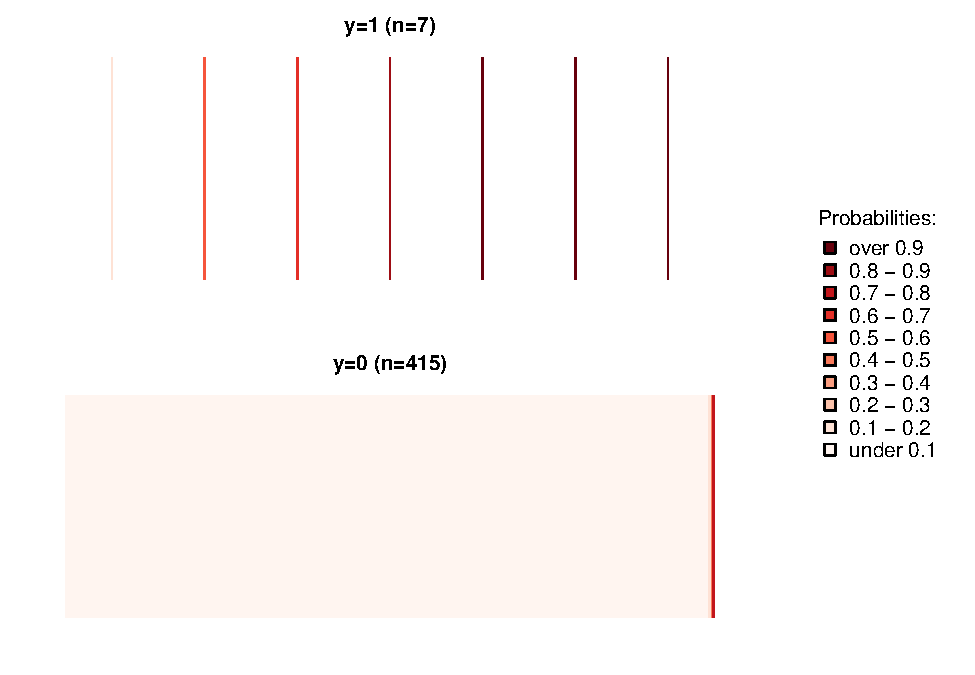
\includegraphics{bookdown-demo_files/figure-latex/unnamed-chunk-79-1.pdf}

\chapter{Modelos de supervivencia}\label{modelos-de-supervivencia}

Hay una serie de preguntas recurrentes al análisis de datos políticos
que aún no hemos cubierto. Muchas veces nos interesa saber por qué
ciertos eventos duran lo que duran, o porqué algunas observaciones duran
más que otras. ¿Por qué la paz es tan duradera entre algunos países
mientras que otros guerrean con frecuencia? ¿Cuál es la probabilidad de
que Turquía ingrese a la ingresar a la Unión Europea en 2018? ¿Por qué
algunos legisladores permanecen en sus cargos por varios periodos
consecutivos mientras que otros no logran reelegirse tan solo una vez?
¿Cuánto demora un sindicato en entrar en huelga durante una crisis
económica?

Todas estas preguntas tienen en común que la duración y el momento de
ocurrencia de un evento son parte de la respuesta que buscamos.
Necesitamos un modelo que nos permita llegar a esta respuesta. Janet
Box-Steffensmeier, la principal referencia en Ciencia Política de este
método, se refiere a ellos a ``modelos de eventos históricos'' aunque
buena parte de la literatura los llama modelos de supervivencia o
modelos de duración. Si bien en la Ciencia Política no son modelos tan
utilizados como uno creería (en el fondo, casi todas las preguntas que
nos hacemos pueden ser reformuladas en una pregunta sobre la duración
del evento), las ciencias médicas han explorado estos métodos en
profundidad, y muchas las referencias que uno encuentra en R sobre
paquetes accesorios a estos modelos son de departamentos bioestadísticos
y médicos. De allí que ``modelos de supervivencia'' sea el nombre más
frecuentemente utilizado para estos modelos, ya que en medicina comenzó
a utilizárselos para modelar qué variables afectaban la sobrevida de sus
pacientes enfermos.

Podemos tener dos tipos de bases de datos para estos problemas. Por un
lado podemos tener una base en formato de panel en el que para un
momento dado nuestra variable dependiente codifica si el evento ha
ocurrido (=1) o no (=0). Así, por ejemplo, podemos tener una muestra de
veinte países para cincuenta años (1965-2015) en los que nuestra
variable de interés es si el país ha implementado una reforma
constitucional. La variable independiente asumirá el valor 1 para el año
1994 en Argentina, pero será 0 para el resto de los años en este país.
Por otro lado, podemos tener una base de datos transversal en la que
cada observación aparece codificada apenas una vez. En este caso
necesitamos, además de la variable que nos dirá si en el periodo de
interés el evento ocurrió o no para cada observación (por ejemplo,
Argentina debería ser codificada como ``1''), una variable extra que
codifique el tiempo de ``supervivencia'' de cada observación, es decir,
cuánto tiempo pasó hasta que finalmente el evento sucedió. Para el caso
de Argentina, esta variable codificará 29 (años), que es lo que demoró
en implementarse una reforma constitucional desde 1965. La elección del
año de partida, como podrá sospechar, es decisión del investigador, pero
tiene un efecto enorme sobre nuestros resultados.

Supongamos que nos hacemos la pregunta que se hizo David Altman: ``¿Por
qué algunos países demoran menos que otros en implementar instancias de
democracia directa?''. Para ello tenemos una base de datos en formato de
panel que parte del año 1900 y que llega a 2016 para 202 países (algunas
observaciones, como la Unión Soviética se transforman en otras
observaciones a partir de un determinado año en que dejan de existir).
Al observar sus datos uno nota algo que probablemente también te suceda
en tu base de datos. Para el año 2016 apenas un pequeño porcentaje de
países había implementado este tipo de mecanismos (27\% para ser más
precisos) pero la base está censurada ya que a partir de ese año no
sabemos que ha ocurrido con los países que aún no han implementado
mecanismos de democracia directa. No todas las observaciones han
``muerto'' aún, ¿cómo saber cuándo lo harán? Ésta es una pregunta
válida, que podremos responder con este tipo de modelos, ya que podemos
calcular el tiempo que demorará cada uno de los países censurados en
nuestra muestra (con la información que le damos al modelo, que siempre
es incompleta).

En nuestra base de datos tendremos, al menos, tres tipos de
observaciones (ver figura x): (a) aquellas que, para el momento en que
tenemos datos ya estaban en la muestra, aunque no siempre sabremos hace
cuanto que ``existen'' (en la base de datos de Altman, por ejemplo,
México ya existía como entidad política en 1900, cuando su base de datos
parte. Sabemos que la Primera República Federal existió como entidad
política desde octubre de 1824, por lo que México sería codificado como
existente a partir de esa fecha). Lo que sí sabemos es que en 2012, por
primera vez, México implementó una iniciativa de democracia directa, lo
que define como positiva la ocurrencia del evento que nos interesa
medir; (b) Algunas observaciones estarán desde el comienzo de la
muestra, y existirán hasta el último momento sin haber registrado el
evento de interés. Tal es el caso, en la muestra de Altman, de Argentina
que ya en 1900 está registrado en la base, y hasta el último año de la
muestra no había registrado instancias de democracia directa, lo que la
transforma en una observación censurada; (c) Algunas observaciones
pueden entrar ``tarde'' en la muestra. Por ejemplo, Eslovenia entra a la
muestra de Altman en 1991, que es cuando se independiza de Yugoslavia.

Figura x. (*) hay que hacer un equivalente propio a esta figura.. en el
que el país 1 entre en t2 a la muestra y el país 4 en t5

(insertar fórmulas a continuación)

Los modelos de supervivencia se interpretan a partir de la probabilidad
de que en un momento dado el evento de interés ocurra dado que no ha
ocurrido aun. Esta probabilidad recibe el nombre de tasa de riesgo.
Partimos sabiendo que tenemos una variable, que llamaremos \(T\), y que
representa un valor aleatorio positivo y que tiene una distribución de
probabilidades (correspondiente a la probabilidad del evento ocurrir en
cada uno de los momentos posibles), que llamaremos \(f(t)\), y que se
puede expresar de manera acumulada, como una densidad acumulada
\(F(t)\). Como dijimos que \(T\) es una variable aleatoria, podemos
calcular su distribución que viene dada por la fórmula, en la que vemos
que \(F(t)\) viene dada por la probabilidad de que el tiempo de
supervivencia \(T\) sea menor o igual a un tiempo específico \(t\).

\(F(t)=\int\limits_0^t f(u)d(u)=Pr(T)\leq t)\)

La función de supervivencia \(\hat S(t)\), que es un concepto clave en
estos modelos, está relacionada a \(F(t)\), ya que

\(\hat S(t)= 1-F(t)=Pr(T\geq t)\)

Es decir, la función de supervivencia es la probabilidad inversa de
\(F(t)\), pues dice respecto a la probabilidad de que el tiempo de
supervivencia \(T\) sea mayor o igual un tiempo \(t\) de interés. Para
el ejemplo concreto de Altman, uno podría preguntarse cuál es la
probabilidad de un país no implementar un mecanismo de democracia
directa (lo que sería equivalente a ``sobrevivir'' a dicha
implementación) siendo que ya ha sobrevivido a los mismos por 30 años. A
medida que más y más países en la muestra van implementando iniciativas
de democracia directa, la probabilidad de supervivencia va disminuyendo.

Los coeficientes de los modelos de supervivencia se suelen interpretar
como tasas de riesgo (o ``hazard rates'' en inglés), que es el cociente
de la probabilidad de que el evento suceda y la función de supervivencia

\(h(t)=\frac{f(t)}{S(t)}\)

Así, la tasa de riesgo indica la tasa a la que las observaciones
``mueren'' en nuestra muestra en el momento \(t\), considerando que la
observación ha sobrevivido hasta el momento \(t\). Veremos más adelante
como en el ejemplo de Altman podemos interpretar los coeficientes de
nuestras regresiones como tasas de riesgo. En definitiva, la tasa de
riesgo \(h(t)\) es el riesgo de que el evento ocurra en un intervalo de
tiempo determinado, que viene dado por

\(f(t)=\lim_{\bigtriangleup x \to 0} \frac {P(t+\bigtriangleup t > T \geq t)}{\bigtriangleup t}\)

\section{El modelo Cox de riesgos
proporcionales:}\label{el-modelo-cox-de-riesgos-proporcionales}

Hay dos tipos de modelos de supervivencia, los llamados modelos
paramétricos y los llamados semi-parametricos. Los primeros son aquellos
que hacen supuestos sobre las características de la población a la que
la muestra pertenece. En este caso, los supuestos son sobre el
``baseline hazard'', es decir, sobre el riesgo de que el evento ocurra
cuando todas nuestras variables independientes son iguales a cero. El
tipo de modelo de surpervivencia más común para esta categoría es el
modelo de Weibull. Por otro lado, los modelos semi-parametricos no hacen
ningún tipo de asunciones sobre la función de base, ya que ésta es
estimada a partir de los datos. El ejemplo más famoso de ésta
especificación es la del modelo de Cox.

El Oxford Handbook sobre metodología política dedica un capítulo entero
a discutir modelos de supervivencia, y en él se toma una posición fuerte
en favor de los modelos semi-parametricos. Por un lado, como no se hacen
presupustos sobre la función del riesgo de base, su estimación es mucho
más precisa. En una estimación paramétrica, elegir un ``baseline
hazard'' equivocado siginificará que todo nuestro trabajo analítico
estará sesgado. La decisión de la forma que adopta la curva de base en
un modelo de Weibull debería estar orientado por razones teóricas de
cuál es el efecto de nuestra variable independiente sobre la
probabilidad de supervivencia de la observación (ver figura x). Sin
embargo, no siempre hay tales presupuestos. Elegir una especificación
por Cox nos ahorra de tomar una decisión tan costosa.

Figura x. diferentes riesgos de base en el modelo de Weibull (dibujar
manualmente)

Una segunda ventaja de los modelos semi-parametricos sobre los
paramétricos tiene que ver con el presupuesto de riesgos proporcionales.
Ambos, modelos paramétricos y semi-parametricos asumen que los riesgos
entre dos individuos cualquiera de la muestra se mantienen constantes a
lo largo de todo su periodo de supervivencia. Es decir, se asume que la
curva de riesgo de cada individuo sigue la misma curva en el tiempo.
Ésta es una asunción cara para trabajos en ciencia política, en los que
las observaciones cambian en el tiempo y se diferencian unas de otras.
Piénsense en el trabajo de Altman, por ejemplo. Uno puede teorizar que
la probabilidad de una iniciativa de democracia directa suceder en el
tiempo estará afectada por el nivel de solidez de sus instituciones
democráticas, que podemos medir con algún tipo de variable estándar como
los 21 puntos de Polity IV o la más reciente medición de V-Dem. Podemos,
entonces, esperar que, a mayor solidez institucional, mayor probabilidad
de implementar mecanismos de democracia directa. Sin embargo los valores
de estas variables no solo difieren ente países, sino que a lo largo del
tiempo estas variables cambian mucho para un mismo país. Piénsese en
Colombia, por ejemplo, que en la variable de V-Dem ``v2x\_polyarchy''
sufrió avances y retrocesos entre 1900 y 2016. Cada vez que el valor de
esta variable cambia, necesariamente cambia la tasa de riesgo de
democracia directa para Colombia, rompiendo el presupuesto de
proporcionalidad de los riesgos (ver figura x).

Figura x. evolución en el tiempo de la variable de V-Dem
``v2x\_polyarchy'' para Colombia (hacer en R)

La ventaja del modelo de Cox sobre sus contrapartes paramétricas es que
existen tests para saber si alguna variable de nuestro modelo rompe el
presupuesto de proporcionalidad de los riesgos, y de esa forma podremos
corregirlo generando interacciones entre estas variables y variables
temporales. De esta forma, permitimos que en nuestro modelo haya dos
tipos de coeficientes: coeficientes constantes en el tiempo, y
coeficientes cambiantes en el tiempo. Por ejemplo, podemos imaginar que
ante un aumento brusco en la calidad de las instituciones democráticas
de un país la tasa de riesgo de implementar democracia directa se
dispare, pero que dicho efecto de desvanezca en el lapso de cuatro o
cinco años. La recomendación dada por el Oxford Handbook para una buena
implementación de modelos de supervivencia es la siguiente. Primero,
dada las ventajas de los modelos semi-paramétricos sobre los
paramétricos, se recomienda el uso de Cox sobre Weibull u otro modelo
paramétrico. Una vez que hemos definido nuestra variable dependiente (el
evento), el tiempo de ``nacimiento'' y de ``muerte'' de cada
observación, podemos especificar nuestro modelo. Los coeficientes, se
recomienda, deben ser interpretados en tasas de riesgo (hazard rates),
lo que exige exponenciar los coeficientes brutos. Una vez que tenemos el
modelo que creemos correcto, en función de nuestras intuiciones
teóricas, es necesario testear que ninguno de los coeficientes viole el
presupuesto de proporcionalidad de los riesgos. Para ello ejecutamos un
test de Grambsch y Therneau, o mediante el análisis de los residuos de
Schoenfeld. Una vez identificados los coeficientes problemáticos,
permitimos que estos interactúen con el logaritmo natural de la variable
que mide la duración del evento. De esta forma, permitimos que haya
coeficientes cuyo efecto se desvanece o se potencia con el tiempo. Una
vez corregidos los coeficientes problemáticos, podemos si, proceder a
interpretar nuestro modelo y la función de supervivencia del modelo.

Código en R

\bibliography{packages,book}


\end{document}
